\chapterimage{orange2.jpg}
\chapterspaceabove{4.75cm} 
\chapterspacebelow{7.25cm} 
\chapter{Relation}
% initialize tikz setting for relation graph
\tikzinitRelation
\section{NBG Set Theory and Binary Relation}
In this chapter, we will discuss further topics on set theory, or more specifically, 
relations. With set as tool, we can categorize things and try to build connections 
between them, like defining a function from a preimage to an image. Relation is a superset
, i.e., generalization of function, which is crucial to topics that we will discuss
later in this chapter.

In real life, relation is referred to as some connections between one person or 
one group of people to the other. 
\begin{enumerate}
    \item Imagine a list of students and their grades in a class. Each student 
    (let's say, by their student ID) is linked to a specific grade. 
    This "student-to-grade" pairing is an example of a functional relation, 
    because every student has one and only one grade assigned.
    \item Consider the relationship "has the same birthday as" among people. If person A has the same birthday as person B, and person B has the same birthday as person C, then person A also has the same birthday as person C. This relationship is an equivalence relation because it's reflexive (everyone has the same birthday as themselves), symmetric (if A shares a birthday with B, then B shares a birthday with A), and transitive (if A shares a birthday with B, and B with C, then A shares a birthday with C).
    \item Think about the books on a shelf organized by height. Each book can be considered as "shorter than or equal to" the book next to it if you move from left to right. This arrangement demonstrates an order relation because it's reflexive (each book is the same height as itself), antisymmetric (if one book is both taller and shorter than another, they must be the same book), and transitive (if one book is shorter than a second, and the second is shorter than a third, then the first book is shorter than the third).
\end{enumerate} 
The notion is still quite similar in the context of
mathematics. From many examples we can see this. Like all the mathematical operations
we have defined, the mapping in a function, congruence...
To sum up, relation is am abstract topic, yet not hard to understand, wince it can be
related to the material world easily. 
\subsection{Class}
Additionally, we introduce a new concept related to set to explain what is relation.
The set theory we discussed in the first part of this book is called \textbf{Naive Set Theory}, which Is
actually not the modern set theory. In many aspects, it is not reliable and causes a lot of issues.
A very famous example is Russell's Paradox initiated by the British Philosopher and Mathematician.

Russell's Paradox illustrates a significant problem in the naive set theory, 
which assumed sets could include themselves. The paradox is encapsulated in whether the 
"set of all sets that do not contain themselves" contains itself. 
If it contains itself, it contradicts its defining property. Conversely, if it does not contain 
itself, then by definition, it must contain itself. This dilemma indicated the limitations 
of the naive set theory approach, leading to contradictions. To address these issues, the 
concept of classes was introduced in \href{https://www.wikiwand.com/en/Von_Neumann%E2%80%93Bernays%E2%80%93G%C3%B6del_set_theory}{\textbf{NBG Set Theory} (von Neumann-Bernays-Gödel set theory)}. 

Classes allow for the conceptualization of collections too large or abstract to be considered as sets, thereby circumventing the paradoxes 
associated with a more naive interpretation of set theory.
\begin{remark}
    An interesting fact is that the von Neumann here is exactly \href{https://www.wikiwand.com/en/John_von_Neumann}{John von Neumann},
    who initiated von Neumann Architecture for computer. It seems that a great Computer Scientist is always also a great Mathematician.
\end{remark}
\begin{definition}[Class]
    A \emph{class} is a collection of objects that are grouped together based on a shared property. 
    Classes differ from sets in that they can represent collections of any size, including 
    those too large to be considered as sets, such as the "class of all sets". 
    This concept is essential for avoiding paradoxes in set theory, 
    allowing the discussion of large and abstract collections that cannot 
    otherwise be accommodated within the framework of sets.
    
    In \textbf{NBG set theory}, a \emph{class} is a collection of sets that can be unambiguously defined by a property that all its members share. Formally, a class $C$ is defined as:
    $$
    C = \{ x : P(x) \}
    $$
    where $P(x)$ is a property or predicate formulable in the language of set theory, applicable to sets $x$. If a class is not a set, it is called a \emph{proper class}. For example, the class of all sets, which cannot be a member of any class, is a proper class.
\end{definition}

\subsubsection*{Distinguishing set and class in NBG and Naive theory}
Naive set theory operates under the general principle that any well-defined collection of objects forms a set. This unrestricted comprehension leads to paradoxes such as Russell's paradox. In contrast, NBG set theory distinguishes between \emph{sets}, which are elements of other classes, and \emph{classes}, which may not necessarily be elements of other classes. 

A key distinction in NBG set theory is that a \emph{set} is a class that is an element of another class, while a \emph{proper class}, such as the class of all sets, cannot be an element of any class. This distinction helps avoid the paradoxes typical of naive set theory by restricting certain collections from being members of other collections.

Furthermore, in NBG, sets form a subclass of classes, meaning all sets are classes but not all classes are sets. This hierarchical structure allows for a more rigorous foundation for set theory, accommodating larger collections like the class of all sets or the class of all ordinal numbers, which themselves cannot be sets due to their extensive size.
We also introduce some of the axioms that is really important for the content here, they are
easy to understand, but are important prerequisite for our further discussion.
\begin{axiom}[Axiom of Extensionality]
    Two classes are equal if and only if they have the same elements.
    Formally, the axiom is expressed as:
    \[
    \forall A \forall B (\forall x (x \in A \leftrightarrow x \in B) \rightarrow A = B)
    \]
    
\end{axiom}

The other Axiom is on creating new classes.
\begin{axiom}[Axiom Scheme of Classification]
    For each open sentence \( P(x) \) there exists a class which consists precisely of those sets which satisfy the condition \( P(x) \).
    
    The class whose existence is postulated by the Axiom is denoted by \( \{x : P(x)\} \); thus 
    \( \{x : P(x)\} \) is a term of the theory NBG and the assertion \( u \in \{x : P(x)\} \) is true if 
    and only if \( u \) is a set and \( P(u) \) is true.
\end{axiom}
\subsubsection*{Properties and Operations of Class}
Since the definition of Class and set are related, there are a lot of overlap in their properties.
The union and intersection of two classes are defined in exactly the same way as the union and intersection of two sets in naïve set theory: if \( A \) and \( B \) are classes, then
\begin{align*}
    A \cup B &= \{x : (x \in A) \vee (x \in B)\}, \\
    A \cap B &= \{x : (x \in A) \wedge (x \in B)\}.
\end{align*}
So a set \( x \) is a member of \( A \cup B \) if and only if it is a member of either \( A \) or \( B \) (or both); \( x \) is a member of \( A \cap B \) if and only if it is a member of both \( A \) and \( B \).

The usual properties of these unions and intersections are established as in naïve set theory. Namely, we have the properties known as idempotence,
\begin{align*}
    \forall X(X \cup X = X), \quad \forall X(X \cap X = X),
\end{align*}
associativity,
\begin{align*}
    \forall X \forall Y \forall Z (X \cup (Y \cup Z) = (X \cup Y) \cup Z), \\
    \forall X \forall Y \forall Z (X \cap (Y \cap Z) = (X \cap Y) \cap Z),
\end{align*}
commutativity,
\begin{align*}
    \forall X \forall Y (X \cup Y = Y \cup X), \quad \forall X \forall Y (X \cap Y = Y \cap X),
\end{align*}
and distributivity,
\begin{align*}
    \forall X \forall Y \forall Z (X \cup (Y \cap Z) = (X \cup Y) \cap (X \cup Z)), \\
    \forall X \forall Y \forall Z (X \cap (Y \cup Z) = (X \cap Y) \cup (X \cap Z)).
\end{align*}

\begin{definition}[Complement of Class]
We write \( x \notin y \) as an abbreviation for \( \neg(x \in y) \). Then for each class \( A \) we define the complement of \( A \) to be the class
\begin{align*}
    \sim A = \{x : x \notin A\}.
\end{align*}
\end{definition}

\begin{definition}[Difference of Classes]
For two classes $A$ and $B$, the difference $A~B$ is defined as:
$$
A\sim B \text{ or } A-B=\{x:(x\in A)\land(x\not\in B)\}=A\cap(\thicksim B).
$$
\end{definition}
Also, note that double negation and De Morgan's Law also work for class.

As what we have discussed in set theory that there exist some empty sets, we also have null class and
universe class.
\begin{definition}[Null Class and Universe Class]
    Empty class $\emptyset$ and universe class $V$ are defined by
    $$\emptyset=\{x:x\neq x\}\ \ \ V=\{x:x=x\}.$$
\end{definition}
Classes also have their exclusive operations, including intersection and union.
\begin{definition}[Intersection and Union of Class(of one single class)]\label{intofclass}
    Let $A$ be a class; the union and intersection of the class $A$ are
    the classes
    $$
    \begin{array}{rcl}\bigcup A&=&\{x:(\exists y)((y\in A)\land(x\in y))\},\\
        \bigcap A&=&\{x:(\forall y)((y\in A)\to (x\in y))\}\end{array}
    $$
    Where $x$ is a set and $y$ is a class.
\end{definition}
Thus a class $C$ belongs to $\bigcup A$ if and only if $C$ is a set and $C$ belongs to at least one of the 
members of $A;C$ belongs to $\bigcap A$ if and only if $C$ is a set and $C$ belongs to every member of $A.$

The definition is quite different from intersection and union of sets, as class is a generalization
of set from higher level abstraction. Also, the intersection and union for sets are binary operations,
while unary for one class. 

Below is a brief comparison.

\textbf{Set Union and Intersection:}
\begin{enumerate}
\item For two sets $A$ and $B$, their union $A \cup B$ is the set of all elements that belong to either $A$ or $B$. Formally: $A \cup B = \{x : x \in A \lor x \in B\}$.
\item For two sets $A$ and $B$, their intersection $A \cap B$ is the set of all elements that belong to both $A$ and $B$. Formally: $A \cap B = \{x : x \in A \land x \in B\}$.
\end{enumerate}

\textbf{Class Union and Intersection:}
\begin{enumerate}
\item For a class $A$, the class union $\bigcup A$ is the set of all elements $x$ such that there exists a class $y$, where $y$ is a member of $A$, and $x$ is an element of $y$. Formally: $\bigcup A = \{x : (\exists y)((y \in A) \land (x \in y))\}$.
\item For a class $A$, the class intersection $\bigcap A$ is the set of all elements $x$ such that for every class $y$, if $y$ is a member of $A$, then $x$ is an element of $y$. Formally: $\bigcap A = \{x : (\forall y)((y \in A) \to (x \in y))\}$.
\end{enumerate}

\textbf{Comparison:}
\begin{enumerate}
\item Set union and intersection operate on two sets, while class union and intersection operate on all member sets of a class.
\item Set union includes elements that are in either $A$ or $B$, while class union includes elements that are in at least one member of $A$.
\item Set intersection includes elements that are in both $A$ and $B$, while class intersection includes elements that are in all members of $A$.
\item The result of set union and intersection is always a set, while the result of class union and intersection is not necessarily a set
, but more likely a class that contains sets.
\end{enumerate}

By comparing these concepts, we can see that class union and intersection are generalizations of set 
operations at a higher level of abstraction. They allow us to perform operations on the member sets of a 
class to obtain new sets, which is particularly useful when studying advanced topics in mathematical 
foundations and set theory.

There are several lemmas related to intersection and union of class.

\begin{lemma}
    $\bigcap \emptyset= V$ and $\bigcup \emptyset= \emptyset.$ 
    \end{lemma}
    \begin{proof}
        Let \( C \) be a class. Then we have
        \[
        C \in \bigcap \emptyset \iff C \text{ is a set and } C \text{ belongs to every member of } \emptyset
        \]
        Since $\emptyset$ does not literally have any member.
        \[
        \iff C \text{ is a set}
        \]
        Any set is a member of universe class
        \[
        \iff C \in V.
        \]
        Thus
        \[
        \bigcap \emptyset = V
        \]
        by the Axiom of Extensionality.

        Again let \( C \) be a class. Then
        \[
        C \in \bigcup \emptyset \iff C \text{ is a set and there is a member } x \text{ of } \emptyset \text{ such that } C \in x
        \]
        \[
        \iff C \in \emptyset
        \]
        (since \( \emptyset \) has no members).

        So
        \[
        \bigcup \emptyset = \emptyset
        \]
        by the Axiom of Extensionality.
    \end{proof}
    The inclusive relation of class is very similar to set.
    \begin{definition}[Inclusion of Classes]
        If \( A \) and \( B \) are classes such that every member of \( A \) is also a member of \( B \), 
        i.e., such that we have
        \[
        \forall x ((x \in A) \to (x \in B)),
        \]
        we say that \( A \) is included in \( B \), \( B \) includes \( A \) or \( A \) is a subclass of 
        \( B \), and we write \( A \subseteq B \) or \( B \supseteq A \). (If \( A \) is a set and 
        \( A \subseteq B \) we say that \( A \) is a subset of \( B \).) If \( A \subseteq B \) and there 
        is at least one set \( b \) such that \( b \in B \) but \( b \not\in A \), we say that \( A \) is 
        properly included in \( B \), \( B \) properly includes \( A \) or \( A \) is a proper subclass of 
        \( B \), and we write \( A \subset B \) or \( B \supset A \).
        \end{definition}

        We can also extend power set to power class.
        For every class \( A \) we define the power class \( P(A) \) of \( A \) to be the class of all subsets of \( A \), i.e., \( P(A) = \{x : x \subseteq A\} \).
        This brings us to another axiom in NBG set theory.
        \begin{axiom}[Power Set Axiom]
        For every set \( x \) there exists a set \( y \) such that \( u \in y \) if and only if \( u \subseteq x \).
        \end{axiom}
        
        The Power Set Axiom thus asserts that every subclass \( u \) of a set \( x \) is actually a set (since it is an element of the set \( y \) whose existence is asserted by the axiom) and furthermore that the power class \( P(x) \) of a set \( x \) is also a set (and so is usually referred to as the power set of \( x \)).
        
        The rest of the axioms are as follows.
        \begin{axiom}[Pairing Axiom]
        For all sets \( x \) and \( y \) the class \( \{z : (z = x) \vee (z = y)\} \) is a set.
        \end{axiom}
        
        The set \( \{z : (z = x) \vee (z = y)\} \) is denoted by \( \{x, y\} \) and such a set is called an 
        unordered pair. If \( x = y \) the unordered pair \( \{x, y\} \) is denoted by \( \{x\} \) and is 
        called singleton \( x \).
        \begin{remark}
            In set theory, an \emph{unordered pair} refers to a collection of two elements in which the sequence of the elements does not matter. This is represented as $\{a, b\}$, indicating a set that contains exactly two distinct elements $a$ and $b$. The fundamental property of unordered pairs is that $\{a, b\} = \{b, a\}$, asserting that the order of elements is immaterial.

The concept of an unordered pair is not limited to sets; it extends to classes in certain set theories that distinguish between sets and proper classes. While sets are collections of elements that themselves can be elements of other sets, proper classes are collections too large to be sets and hence cannot be elements of other collections. Nonetheless, the notion of grouping two objects into an unordered pair applies analogously, symbolizing the collection of those objects without regard to order.
        \end{remark}
        \begin{axiom}[Union Axiom]
        For every set \( x \) the class \( \bigcup x \) is a set.
        \end{axiom}

        We can also extend Cartesian Product to class.
        Let $a$ and $b$ be sets. Then the set $\{\{a\},\{a,b\}\}$ is denoted by $(a,b)$ and is called the ordered pair with first coordinate $a$ and second coordinate $b$. Lét $A$ and $B$ be classes; then the Cartesian product of $A$ and $B$ is the $c$lass

        $$
        A\times B=\{t:(\exists x)(\exists y)((x\in A)\land(y\in B)\land(t=(x,y)))\},
        $$

        i.e. $A\times B$ is the class of all ordered pairs with first coordinate in $A$ and second coordinate in $B.$

        If $P(x,y)$ is an open sentence involving the free variables $x$ and $y$ we shall allow ourselves to write

        $$
        \{(x,y):P(x,y)\}
        $$

        as an abbreviation for

        $$
        \{t:(\exists x)(\exists y)((t=(x,y))\land P(x,y))\}.
        $$

        So we can abbreviate the definition of $A\times B$ to

        $$
        A\times B=\{(x,y):(x\in A)\wedge(y\in B)\}.
        $$


\subsection{Binary Relations, Composition and Inverse}
In mathematics, the most fundamental and ubiquitous type of relation is the \emph{binary relation}. This term refers to a relationship between two objects or sets. We understand that a `set' may encompass any concept, not solely in the mathematical sense but also in a material one. Relations may exist objectively between certain objects and not at all for others. Similarly, objects or sets of objects, which exist objectively, hold the potential for an infinite number of relationships with one another. This perspective can seem philosophically abstract, positing that any scenario is conceivable. However, we can convey this more clearly. Recall our discussion of the \emph{Cartesian product} as a set extension, where we consider two sets, \( A \) and \( B \). These sets could represent any discernible entity or indiscernible concept. Theoretically, there could be countless relationships among all elements of these sets, and the capacity of two sets to form a Cartesian product is indicative of a general type of relationship. Consequently, the elements of the power set \( P(A \times B) \) exemplify all possible cases of a certain kind of relationship.

A vivid mathematical example is the definition of Euclidean spaces, where an infinite number of subspaces can be defined, each representing a unique binary relation within the space.

We first introduce the definition of a binary relation in terms of sets. 
\begin{definition}[Binary Relation]
    A \textbf{Binary Relation} $R$ from a set $A$ to a set $B$ is a subset of the 
    Cartesian product $A \times B$. For elements $a \in A$ and $b \in B$, if the pair 
    $(a, b)$ belongs to the subset $R$, then we say $a$ is related to $b$ by the 
    relation $R$, denoted as $aRb$, whose negation is $a\not R b$.
\end{definition}

In last section, we introduced the higher abstraction of sets, which is class. Classes also have Cartesian
product,thus, we can give a general definition to all relations using class.
\begin{definition}[Relation]
    A relation is a class of ordered pairs.

    Let $R$ be a relation. We define the domain and range of $R$ to be the classes Dom $R$ and Range $R$ 
    given by
$$
\begin{array}{rcl}\text{Dom }R&=&\{x:(\exists y)((x,y)\in R)\},\\\text{Range }R&=&\{y:(\exists x)((x,y)\in R)\}.\end{array}
$$
If $R$ is a relation and $(x,y)\in R$ we say that $x$ is $R$-related to $y$ and that $y$ is an $R$-relative of $x$. 
Thus Dom $R$ is the class of all sets which $have$ $R$-relatives and Range $R$ is the class of all sets which 
$are$ $R$-relatives.
\end{definition}

Now we look into several concrete examples of relation.
\begin{example}
    Consider the set of all points on a plane. The relation defined by the equation of a circle, $x^2 + y^2 = r^2$, includes all points $(x, y)$ that satisfy this equation. This relation is not a function because, for most values of $x$, there are two possible values of $y$ that satisfy the equation, one positive and one negative (except for the points where $x = \pm r$, where there is only one value of $y$).
    
    In contrast, a function would allow each $x$ to be associated with exactly one $y$. For instance, the square function $y = x^2$ is a function because each value of $x$ corresponds to exactly one value of $y$.

    In the figure we have defined a circle and a quadratic function, clearly 
    we see that a function can never have two $y$ value for one $x$, while 
    this is possible for the circle.
    \end{example}
\begin{figure}[H]
    \centering
    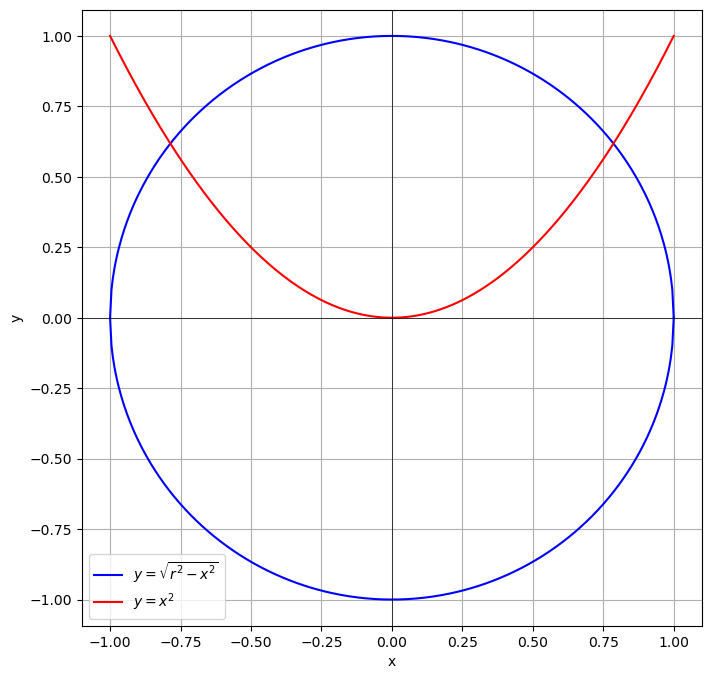
\includegraphics[width = 0.75\linewidth]{function&relation.png}
    \caption{Visual Comparison of a Relation and a Function}
\end{figure}
\begin{example}
	Let A be the set \{1,2,3,4\}. Which ordered pairs are in the relation $R=\{(a,b)\mid a$ divides $b\}?$
	\begin{solution}
		 Because $(a,b)$ is in R if and only if $a$ and $b$ are positive integers not exceeding 4 such that $a$ divides $b$,we see that
		$$
		R=\{(1,1),(1,2),(1,3),(1,4),(2,2),(2,4),(3,3),(4,4)\}.
		$$
	\end{solution}
\begin{figure}[H]
	\centering
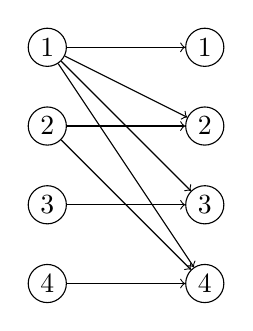
\begin{tikzpicture}
	
	% Define style for the nodes
	\tikzstyle{number}=[circle, draw, inner sep=2pt]
	
	% Draw nodes
	\node[number] (1l) at (0,3) {1};
	\node[number] (2l) at (0,2) {2};
	\node[number] (3l) at (0,1) {3};
	\node[number] (4l) at (0,0) {4};
	
	\node[number] (1r) at (2,3) {1};
	\node[number] (2r) at (2,2) {2};
	\node[number] (3r) at (2,1) {3};
	\node[number] (4r) at (2,0) {4};
	
	% Draw arrows
	\draw[->] (1l) -- (1r);
	\draw[->] (1l) -- (2r);
	\draw[->] (1l) -- (3r);
	\draw[->] (1l) -- (4r);
	
	\draw[->] (2l) -- (2r);
	\draw[->] (2l) -- (4r);
	
	\draw[->] (3l) -- (3r);
	
	\draw[->] (4l) -- (4r);
\end{tikzpicture}
\caption{$R=\{(a,b)\mid a$ divides $b\}$}
\end{figure}
This relation also differs from function, since for member of $a$, it is possible
to map to multiple members in $b$.
\end{example}
\begin{definition}[Functional Relation]
    A relation $R$ is said to be \textbf{functional} if each element of its domain has exactly one $R$-relative; 
    a functional relation is also called a \textbf{function}. If $R$ is a functional relation then for each element 
    $a$ of its domain we denote the unique $R$-relative of $a$ by $R(a).$ 
\end{definition}

    This leads us to the next axiom of NBG theory.
    \begin{axiom}[Replacement Axiom]
        For every functional relation $R$, if the domain of $R$ is a set then the range 
        of $R$ is also a set.
    \end{axiom}
\subsection{Mapping, Composition, and Inverse}
    In naive set theory and function in part 1 of the book, we gave a rough 
    definitions to mappings. With class, we can make it more concrete.
    \begin{definition}[mapping]
        A mapping is an ordered pair $((A,B),R)$ where $A$ and $B$ are sets and $R$ is a 
        functional relation between $A$ and $B$ such that Dom $R=A.$ If 
        $f= ( ( A, B) , R) $ is a mapping we say that $f$ is a mapping from 
        $A$ to $B;$ we call $A$ the domain of $f,B$ the codomain of $f$ and $R$ the 
        graph of $f$. If $f$ is a mapping with domain $A$ and codomain $B$ we often write $f:A\to B.$ 
        If $a$ is any element of the set $A$ then the set $R^{\to}(\{a\})$ consists of a single element of 
        $B$ which we denote by $f(a);$ we call it the image of $a\textbf{ under }f$ or the value of $f\textbf{ at }a.$
    \end{definition} 
    It is clear from the definition of the term “mapping” that in order to describe a mapping $f$ we must give the domain $A$ and codomain $B$ of $f$ and also, for each element $a$ of the domain we must describe the unique element $b_a$ of the codomain such that $(a,b_a)$ belongs to the graph of $f$, i.e. we must describe for each element $a$ of $A$ its image under $f$ in $B.$
    
    Let $f= ( ( A, B) , R) $ be a mapping from $A$ to $B$. For each subset $X$ of $A$ we denote the subset 
    $R^{\to}(X)$ of $B$ by $f^{\to}(X);$ in particular, if $a$ is any element of $A$ we have
    $f^{\to}(\{a\})=\{f(a)\}.$ For each subset $Y$ of $B$ we denote the subset $R^{\leftarrow }( Y) $ 
    of $A$ by $f^{\leftarrow }( Y) .$

    Let $ f=((A,B),R)$ be a mapping from $A$ to $B;\operatorname*{let}A_1$ be a subset of $A.$ Then the restriction of $f$ to $A_1$ is the mapping
    $$
    f\mid A_1= \left((A_1,B\\),R\cap(A_1\times B)\right).
    $$

    Earlier, we discussed composition and inverse of function. Now that we have known that function is a kind of 
    relation, can we compose or inverse all other relations? Naturally the answer is yes.
	
	\begin{definition}[Special Mappings]
		Let $f= ( ( A, B) , R) $ be a mapping. Then $f$ is said to be \textbf{surjective} or to be a \textbf{surjection} if we have
		Range $R$ $= B, $i.e. if every element of $B$ is the image under $f$ of at least one element of $A.$
		
		Next, $f$ is said to be \textbf{injective} or to be an \textbf{injection} if the inverse relation $R^{-1}$ is functional. Thus $f$ is an injection if and only if for every element $b$ in Range $R$ there is exactly one element $a$ of $A$ such chat $( b, a) \in R^{- 1}, $i.e.$\quad ( a, b) \in R$ and so $b=f(a).$ So $f$ is injective if and only if each element of the range of $R$ is the image under $f$ of exactly one element of $A.$ Again, $f$ is injective if and only if whenever $f( a_{1}) = f( a_{2}) , $ where $a_{1}, a_{2}\in A, $ then $a_{1}= a_{2}.$
		
		The mapping $f$ is said to be \textbf{bijective} or to be a \textbf{bijection} if it is both injective and surjective. If $A$ and $B$ are sets we say that $A\textbf{is}$ equipotent to $B$ or that $A\textbf{is equinumerous with }B$ if there exists a bijective mapping from $A$ to $B.$
		
		Let $f=((A,B),R)$ be a mapping. Then $((B,A),R^{-1})$ is a mapping if and only if $f$ is bijective; in this case we write $((B,A),R^{-1})=f^{-1}$ and call $f^{-1}$ the inverse mapping of $f.$ Clearly $f^{-1}$ is a bijection from $B$ to $A$ with inverse $f.$
		\end{definition}
		Here are some examples of special mappings.
		\begin{example}[Surjective Function]
			A function \( f: A \to B \) is surjective if for every element \( y \) in \( B \), there is at least one element \( x \) in \( A \) such that \( f(x) = y \). For instance, let \( A = \{1, 2, 3\} \) and \( B = \{a, b\} \). Define \( f \) by \( f(1) = a \), \( f(2) = a \), and \( f(3) = b \). This function is surjective because every element of \( B \) is the image of at least one element of \( A \).
		\end{example}
		
		\begin{example}[Injective Function]
			A function \( f: A \to B \) is injective if no two different elements in \( A \) map to the same element in \( B \). For example, let \( A = \{1, 2, 3\} \) and \( B = \{a, b, c, d\} \). Define \( f \) by \( f(1) = a \), \( f(2) = b \), and \( f(3) = c \). This function is injective because each element of \( A \) maps to a unique element of \( B \).
		\end{example}
		
		\begin{example}[Bijective Function]
			A function \( f: A \to B \) is bijective if it is both injective and surjective. For instance, let \( A = \{1, 2, 3\} \) and \( B = \{a, b, c\} \). Define \( f \) by \( f(1) = a \), \( f(2) = b \), and \( f(3) = c \). This function is bijective, making \( A \) and \( B \) equinumerous.
		\end{example}
		
		\begin{example}[Inverse Mapping]
			If \( f \) is a bijective function from \( A \) to \( B \), then the inverse \( f^{-1} \) is a function from \( B \) to \( A \) that reverses the mapping of \( f \). Using the bijective function \( f \) from the previous example, we define \( f^{-1} \) by \( f^{-1}(a) = 1 \), \( f^{-1}(b) = 2 \), and \( f^{-1}(c) = 3 \).
		\end{example}
		
	
    \begin{definition}[Composite Relation]
        If $R$ and $S$ are relations, the composition of $R$ and $S$ is the relation $S\circ R$ given by
        $$
        S\circ R=\{(x,z):(\exists y)(((x,y)\in R)\wedge((y,z)\in S))\}.
        $$
        If $R$ is a relation between $A$ and $B$ and $S$ is a relation between $B$ and $C$ then clearly 
        $S\circ R$ is a relation between $A$ and $C$, and we have $\operatorname{Dom}\left(S\circ R\right)\subseteq\operatorname{Dom}R$ and Range $(S\circ R)\subseteq\operatorname{Range}S.$
    \end{definition}
    The idea of composition also works for mappings.
\begin{definition}[Composite Mapping]
    Let $f= ( ( A, B) , R) $ and $g= ( ( B, C) , S) $ be mappings. Then clearly 
    $((A,C),S\circ R)$ is also a mapping, which we denote by $g\circ f$ and call the composition or 
    composed mapping of $f$ and $g$. For each element $a$ of $A$ we have $( g\circ f) ( a) = g( f( a) ).$

\end{definition}
\begin{remark}
	The other equivalent definition is that
	Let $R$ be a relation from a set $A$ to a set $B$ and S a relation from $B$ to a set $C$. The $composite$ of $R$ and S is the relation consisting of ordered pairs $(a,c)$, where $a\in A, c\in C$ , and for which there exists an element $b\in B$ such that $( a, b) \in R$ and $( b, c) \in S.$ We denote the composite of $R$ and $S$ by $S\circ R.$
\end{remark}
    Similarly, we can define inverse relation.
    \begin{definition}[Inverse Relation]
        If $A$ and $B$ are classes then a relation between $A\textbf{ and }B$ is a subclass of $A\times B$, 
        i.e. a relation $R$ such that Dom $R\subseteq A$ and Range $R\subseteq B.$ A relation on a class $A$ 
        is a subclass of $A\times A.$

        If $R$ is a relation, the inverse of $R$ is the relation $R^{-1}$ given by
        $$
        R^{-1}=\{(x,y):(y,x)\in R\}.
        $$
        If $R$ is a relation between $A$ and $B$ then $R^{-1}$ is a relation between $B$ and $A;$ 
        clearly Dom $R^{-1}=\operatorname{Range}R$ and Range $R^{-1}=\operatorname{Dom}R.$
    \end{definition}

    Let $R$ be a relation, $A$ any class. Then the image of $A\textbf{ under }R$ is the class consisting of all $R$-relatives of all members of $A.$ We denote this class by $R^{\to}(A).$ Thus
    $$
    R^{\to}(A)=\{y:(\exists x)((x\in A)\land((x,y)\in R))\}.
    $$
    Again let $R$ be a relation and $\ker B$ be any class. Then the inverse image of $B$ under $R$ is the class $( R^{- 1}) ^{\to }( B) , $ which we write $R^{\leftarrow}( B) .$ Thus
    $$
    \begin{aligned}R^{\leftarrow}(B)=\{x:(\exists y)((y\in B)\land((x,y)\in R))\}.\end{aligned}
    $$
    With functional relation and mapping, we can define a more specific relation, which very special and practical.
    \begin{definition}[Diagonal (Relation) and Identity Mapping]\label{diagonalR}
    	Let $A$ be any set; let $D_A=\{x:(\exists a)((a\in A)\land(x=(a,a)))\}$ (we call $D_A$ the diagonal of $A\times A).$ Then $D_A$ is a functional relation between $A$ and $A$ with domain $A.$ The mapping $I_A=((A,A),D_A)$ from $A$ to $A$ is called the identity mapping of $A.$ Clearly we have $I_{A}(a)=a$ for each element $a$ of $A.$
    \end{definition}
   \begin{example}
   	The identity mapping $I_A$ for a set $A$ is a function that maps every element to itself. Here are some examples of identity mappings on various sets:
   	
   	\begin{itemize}
   		\item Let $B = \{x \in \mathbb{R} \mid -1 \leq x \leq 1\}$. The identity mapping on $B$ is $I_B : B \to B$ where $I_B(x) = x$ for all $x \in B$.
   		
   		\item Let $C = \{\text{apple}, \text{banana}, \text{cherry}\}$. The identity mapping on $C$ is $I_C : C \to C$ where $I_C(\text{fruit}) = \text{fruit}$ for each fruit in set $C$.
   		
   		\item Let $D = \mathbb{Z}$. The identity mapping on $D$ is $I_D : \mathbb{Z} \to \mathbb{Z}$ where $I_D(n) = n$ for all $n \in \mathbb{Z}$.
   	\end{itemize}
   	
   	The diagonal for each of these sets would be as follows:
   	\begin{itemize}
   		\item The diagonal of $B$, $D_B$, would be the set of all ordered pairs $(x, x)$ such that $x \in B$.
   		
   		\item The diagonal of $C$, $D_C$, would be the set $\{(\text{apple}, \text{apple}), (\text{banana}, \text{banana}), (\text{cherry}, \text{cherry})\}$.
   		
   		\item The diagonal of $D$, $D_D$, would be the set of all ordered pairs $(n, n)$ such that $n \in \mathbb{Z}$.
   	\end{itemize}
   	
   	In all these cases, the identity mapping illustrates the concept of a function where the input is the same as the output for each element of the set.
   \end{example}
\subsection{Families of Sets}
In part 1, we discussed sequence. Sequence is defined (see definition \ref{def_sequence}) by a relation between index and a mathematical expression related to the index, and commonly the index $i$ has $i\in \N$. Sequence is actually a special \textbf{family of set}.
\begin{definition}[Family of Set]
	Let $I$ and $A$ be classes, and $F$ is a functional relation between $I$ and $A$. Then $F$ is sometimes called a family of elements of $A$ indexed by $I$ (or with $I\textbf{ as index class}) $ and we write $(F(i))_{i\in I}$ instead of $F$. In particular, if $E$ is a set then a family of elements of $\mathbf{P}(E)$ is called a family of subsets of $E$ indexed by $I.$ If $F$ is such a family and we write $X_i=F(i)$ for each element $i$ in $I$ then we denote the family $F$ by$\left ( X_i\right ) _{i\in I}.$
\end{definition} 
If $X$ is a set of subsets of a set $E$ then the diagonal $D_X$ is a family of subsets of $E$ which may sometimes be denoted by $(x)_{x\in X}.$

Let $F= ( X_{i}) _{i\in I}$ be a family of subsets of a set $E.$ We define the union of the family to be
$$
\bigcup_{i\in I}X_i=\{x:(\exists i)((i\in I)\land(x\in X_i))\}.
$$
Thus $x$ belongs to the union of the family $(X_i)_{i\in I}$ if and only if it belongs to at least one of the sets $X_i$ with $i$ in $I.$ Of course if $X$ is a set of subsets of $E$ the union of the corresponding family $D_X$ coincides with the union of the set $X$ as previously defined: $\bigcup_{x\in X}x=\bigcup X.$

Again let $(X_i)_{i\in I}$ be a family of subsets of a set $E.$ The intersection of this family is defined to be
$$
\bigcap_{i\in I}X_i=\{x:(x\in E)\land(\forall i)((i\in I)\Longrightarrow(x\in X_i))\}.
$$
So $x$ belongs to the intersection of the family $(X_i)_{i\in I}$ if and only if it belongs to all the sets $X_i$ with $i$ in $I.$

We notice that if $I$ is empty then we have $\bigcap_{i\in I}X_i=E.$ If X i a non-empty set of subsets of $E$ the intersection of the corresponding family $D_X$ coincides with the intersection of the set $X$ as previously defined${: }\bigcap _{x\in X}x= \bigcap X.$
\begin{example}
Consider the set $E$ and a family of its subsets $(X_i)_{i \in I}$, where $I = \{1, 2, 3\}$ and
\begin{itemize}
	\item $X_1 = \{a, b\}$
	\item $X_2 = \{b, c\}$
	\item $X_3 = \{a, c, d\}$
\end{itemize}

The union of the family $(X_i)_{i \in I}$ is the set of elements that are in at least one of the sets $X_i$:
\[ \bigcup_{i \in I} X_i = X_1 \cup X_2 \cup X_3 = \{a, b, c, d\} \]

The intersection of the family $(X_i)_{i \in I}$ is the set of elements that are in every one of the sets $X_i$:
\[ \bigcap_{i \in I} X_i = X_1 \cap X_2 \cap X_3 = \emptyset \]
\end{example}

\begin{definition}[Sequence as Family of Set]
Let \( E \) be a set. A sequence in \( E \) is a function from the set of natural numbers \( \mathbb{N} \) to \( E \). The sequence can be represented as a family of sets \( (x_i)_{i \in \mathbb{N}} \), where each \( x_i \) is an element of \( E \), and \( i \) is the index representing the position of the element in the sequence.

The \( n \)-th term of the sequence is denoted by \( x_n \), and the sequence itself can be written as \( (x_n)_{n=1}^{\infty} \), which is the family of elements of \( E \) indexed by \( \mathbb{N} \).
\end{definition}

Let $(X_i)_{i\in I}$ be a family of sets with index set $I.$ Let $X=\bigcup_{i\in I}X_i.$ Then the product of the family $(X_i)_{i\in I}$ is the set

$$
\prod_{i\in I}X_i=\{f:(f\in\operatorname{Map}(I,X))\wedge(\forall i)((i\in I)\Longrightarrow(f(i)\in X_i))\}.
$$
If we write $f(i)=x_i$ for each index $i$ in $I$ it is sometimes helpful to denote the element $f$ of $\prod_{i\in I}X_i$ by $\prod_{i\in I}x_i.$

For each index $j$ in $I$ we define a mapping $\pi_j$ from $\prod_{i\in I}X_i$ to $X_j$ by setting

$$
\pi_j(f)=f(j)\text{ for every }f\mathrm{~in~}\prod_{i\in I}X_i.
$$

The mapping $\pi_j$ is called the $j$ -th projection mapping from $\prod_{i\in I}X_i.$
\begin{example}
	Consider two sets $X_1 = \{a, b\}$ and $X_2 = \{1, 2\}$. The index set is $I = \{1, 2\}$.
	The product of the family of sets $(X_i)_{i \in I}$, which is $X_1 \times X_2$, consists of all ordered pairs where the first element is from $X_1$ and the second is from $X_2$. Thus, the product is:
	\[ \prod_{i \in I} X_i = X_1 \times X_2 = \{(a, 1), (a, 2), (b, 1), (b, 2)\} \]
	
	Each ordered pair represents a function $f$ mapping $I$ to the union of $X_1$ and $X_2$. For instance, one such function corresponding to the ordered pair $(a, 1)$ is defined by:
	\[ f(1) = a, \quad f(2) = 1 \]
	
	Projection mappings $\pi_j$ from $\prod_{i \in I} X_i$ to $X_j$ are defined for each index $j \in I$ by setting:
	\[ \pi_1(f) = f(1), \quad \pi_2(f) = f(2) \]
	
	Hence, for our function $f$, the projections are:
	\[ \pi_1(f) = a, \quad \pi_2(f) = 1 \]
\end{example}

Family of Sets is related to another axiom of NBG set theory.
\begin{axiom}[Axiom of Choice]
	 Let $(E_i)_{i\in I}$ be a family of nonempty sets indexed by a set $I$. Then the product $\prod_{i\in I}E_i$ is non-empty.
\end{axiom}
We can also define choice function of class.
\begin{definition}[Choice Function and Selection Set]
	Let $(E_i)_{i\in I}$ be a family of non-empty sets. By a \textbf{choice function} for this family we mean a mapping $f$ from $I$ to $\bigcup_{i\in I}E_i$ such that for every index $i$ in $I$ we have $f(i)\in E_i;$ thus a choice function is an element of the product $\prod_{i\in I}E_i.$ If we have $E_i\cap E_j=\emptyset$ for every pair of distinct elements $i, j$ of $I$ we say that the family $( E_i) _{i\in I}$ is $pairwise$ $disjoint)$ then the range of a choice function for $(E_i)_{i\in I}$ is a subset of $\bigcup_{i\in I}E_i$ which contains exactly one element from each set of the family. Such a set is called a \textbf{selection set} for the (pairwise disjoint) family $(E_i)_{i\in I}.$
\end{definition}
Thus the Axiom of Choice asserts that for every family of non-empty
sets there exists a choice function and so for every pairwise disjoint family
of non-empty sets there exists a selection set.
\begin{example}[Choice Function and Selection Set]
	Consider the family of non-empty, pairwise disjoint sets:
	\begin{align*}
		E_1 &= \{1, 2\}, \\
		E_2 &= \{3, 4\}, \\
		E_3 &= \{5, 6\},
	\end{align*}
	with the index set \( I = \{1, 2, 3\} \).
	
	A choice function \( f \) for this family might be defined as:
	\begin{align*}
		f(1) &= 1, \\
		f(2) &= 4, \\
		f(3) &= 5.
	\end{align*}
	This function \( f \) chooses one element from each set \( E_i \), making the selection set for this family \(\{ f(1), f(2), f(3) \} = \{1, 4, 5\}\).
\end{example}
\subsection{Reflexivity, Symmetry, and Transitivity}
With basic relation we have defined, we can now look into some special relations with some specific properties. These properties are important, since these property will be used to further classify relations for us. All special relations could be related to the diagonal of the sets or classes involved in that specific relation.

The first special relation is actually already covered in the diagonal of class, which is the idea of reflexivity, meaning a relation from an object to itself.
\begin{definition}[Reflexive Relation]\label{reflexR}
	Let \( R \) be a relation on a set \( X \). The relation \( R \) is said to be \textbf{reflexive} if \( D_X \subseteq R \), where \( D_X = \{(x, x) \mid x \in X\} \). That is, for every element \( x \) in \( X \), the pair \( (x, x) \) belongs to \( R \).
\end{definition}
\begin{example}
	Consider the following relations on the set \(\{1, 2, 3, 4\}\):
	
	\begin{itemize}
		\item \( R_1 = \{(1, 1), (1, 2), (2, 1), (2, 2), (3, 4), (4, 1), (4, 4)\} \)
		\item \( R_2 = \{(1, 1), (1, 2), (2, 1)\} \)
		\item \( R_3 = \{(1, 1), (1, 2), (1, 4), (2, 1), (2, 2), (3, 3), (4, 1), (4, 4)\} \)
		\item \( R_4 = \{(2, 1), (3, 1), (3, 2), (4, 1), (4, 2), (4, 3)\} \)
		\item \( R_5 = \{(1, 1), (1, 2), (1, 3), (1, 4), (2, 2), (2, 3), (2, 4), (3, 3), (3, 4), (4, 4)\} \)
		\item \( R_6 = \{(3, 4)\} \)
	\end{itemize}
	
	Which of these relations are reflexive?
	
	\textbf{Solution:} The relations \( R_3 \) and \( R_5 \) are reflexive because they both contain all pairs of the form \( (a, a) \), namely, \( (1, 1), (2, 2), (3, 3), \) and \( (4, 4) \). The other relations are not reflexive because they do not contain all of these ordered pairs. In particular, \( R_1, R_2, R_4, \) and \( R_6 \) are not reflexive because \( (3, 3) \) is not in any of these relations.
\end{example}
And as a complement of Reflexivity, we can define Irreflexivity
\begin{definition}[Irreflexive Relation]
	A relation \( R \) on a set \( X \) is called \textbf{irreflexive} if \( D_X \cap R = \emptyset \), i.e., no pair of the form \( (x, x) \) belongs to \( R \) for any \( x \) in \( X \).
\end{definition}

Now we discuss symmetry of relation.
\begin{definition}[Symmetric Relation]
	A relation \( R \) on a set \( X \) is \textbf{symmetric} if for every \( x, y \) in \( X \), if \( (x, y) \in R \) then \( (y, x) \) is also in \( R \), i.e., $R = R^{-1}$
\end{definition}

We can also define the complement of this kind of relation.
\begin{definition}[Asymmetric Relation]
	Let \( R \) be a relation on a set \( X \). The relation \( R \) is said to be \textbf{asymmetric} if for any \( x, y \) in \( X \), whenever \( (x, y) \in R \), then \( (y, x) \notin R \). This implies that no pair can be in both \( R \) and \( R^{-1} \) unless \( x = y \), which is not permitted for asymmetric relations, thus \( R \cap R^{-1} = \emptyset \), i.e. $R \neq R^{-1}$, .
\end{definition}
There is also a type of relation called antisymmetric relation.
\begin{definition}[Antisymmetric Relation]
	A relation \( R \) on a set \( X \) is \textbf{antisymmetric} if for all \( x, y \) in \( X \), if \( (x, y) \in R \) and \( (y, x) \in R \), then \( x = y \). That is, \( R \cap R^{-1} \subseteq D_X \).
\end{definition}
Some may confused by these similar terms. Below are the clarification and some examples.
\begin{itemize}
	\item A relation \( R \) on a set \( X \) is \textbf{symmetric} if for any \( x, y \in X \), whenever \( (x, y) \) is in \( R \), then \( (y, x) \) is also in \( R \). Symmetry implies a mutual relationship.
	
	\item A relation \( R \) is \textbf{asymmetric} if for any \( x, y \in X \), whenever \( (x, y) \) is in \( R \), \( (y, x) \) is not in \( R \). Asymmetry denotes a one-way relationship.
	
	\item A relation \( R \) is \textbf{antisymmetric} if for any \( x, y \in X \), whenever both \( (x, y) \) and \( (y, x) \) are in \( R \), it must be that \( x = y \). Antisymmetry allows for a hierarchical ordering.
\end{itemize}

Let's explore these properties through examples:

\begin{example}[Symmetric Relation]
	The relation "is a sibling of" is symmetric. If Tom is a sibling of Jerry, then Jerry is a sibling of Tom.
\end{example}

\begin{example}[Asymmetric Relation]
	The "less than" relation on the real numbers is asymmetric. If \( 3 < 4 \), then it is not the case that \( 4 < 3 \).
\end{example}

\begin{example}[Antisymmetric Relation]
	The "divides" relation for integers is antisymmetric. For example, \( 6 \) divides \( 12 \), and \( 12 \) does not divide \( 6 \). But we can have 6 divides 6 itself.
\end{example}
\subsection{Exercises}



\begin{exercise}
	 Determine whether each of the following is a set or a class in NBG set theory, and explain why.
	\begin{enumerate}
		\item The collection of all sets that do not contain themselves.
		\item The set of all natural numbers.
		\item The class of all ordinal numbers.
	\end{enumerate}
\end{exercise}
\begin{solution}
	Below are the solutions.
	\begin{enumerate}
		\item The collection of all sets that do not contain themselves is a \textbf{proper class}. This is because any attempt to consider it as a set leads to Russell's paradox, thus it cannot be a set within any consistent set theory including NBG.
		\item The set of all natural numbers is a \textbf{set}. It is well-defined and does not lead to any paradoxes within NBG set theory. Furthermore, it is an element of the class of all sets.
		\item The class of all ordinal numbers is a \textbf{proper class} because it is too large to be a set. If it were a set, it would lead to contradictions similar to those arising from considering the "set of all sets."
	\end{enumerate}
\end{solution}
\begin{exercise}
    Russel's Paradox is fixed by introducing more strict set axioms to the set theory. In NBG theory, a
    proper class is defined as a top-level class that cannot be subclass of any other classes or sets, and
    this is the key to avoid the paradox in naive set theory. Explain in details that how 
    this concept avoids the case in Russel's Paradox.
\end{exercise}
\begin{solution}
    With the introduction of the concept of classes, we can discuss collections 
    that are too large to be considered as sets, such as the ``class of all sets.'' 
    Therefore, the set described by Russell's Paradox, denoted by \( R \), 
    is no longer considered a legitimate set but rather a ``proper class.'' 
    This means that we refrain from discussing \( R \) as a set, thereby avoiding 
    the paradox because proper classes are not subject to the operations and 
    axioms that constrain sets. As a result, the axiomatic system does not 
    permit the formation of sets that would lead to Russell's Paradox.

\end{solution}
\begin{exercise}
    Let $A,B,C$ be classes such that $A\subseteq B,B\subseteq C$, $C\subseteq A.$ Prove that $A=B=C.$
\end{exercise}

\begin{exercise}
    Let $A,B,C$ be classes such that $A\subset B,B\subset C.$ Prove that $A\subset C.$
\end{exercise}

Below are exercises for binary relation.




\section{Representation of Relations}
In last section. we discussed binary relation and their properties. This section focuses on ways of representation. Symbolic language is accurate and not prone to make misunderstanding, yet it is not quite easy to understand to human minds. Therefore, we need straightforward ways to visualize them and assure the accuracy in the same time.
	\subsection{Representation By Matrix}
	The first commonly used method is matrix. A relation between finite sets can be represented using a zero-one matrix. Suppose that $R$ is a relation from $A=\{a_1,a_2,\ldots,a_m\}$ to $B=\{b_1,b_2,\ldots,b_n\}.$ (Here the elements of the sets $A$ and $B$ have been listed in a particular, but arbitrary, order. Furthermore, when $A=B$ we use the same ordering for $A$ and $B.)$ The relation $R$ can be represented by the matrix $\mathbf{M}_R=[m_{ij}]$, where
	$$
	m_{ij}=\left\{\begin{matrix}1\text{ if}(a_i,b_j)\in R,\\0\text{ if}(a_i,b_j)\notin R.\end{matrix}\right.
	$$
	\begin{example}
		Consider the binary relation \( R \) on the set \( X = \{1, 2, 3\} \) defined by the pairs \( R = \{(1, 2), (2, 3), (3, 1)\} \). We can represent \( R \) as a matrix \( M \) where the entry \( m_{ij} \) is 1 if \( (i, j) \in R \) and 0 otherwise. Thus, the matrix \( M \) representing \( R \) is given by:
		$$
		M = \begin{bmatrix}
			0 & 1 & 0 \\
			0 & 0 & 1 \\
			1 & 0 & 0
		\end{bmatrix}
		$$
		This matrix shows that there is a relation from 1 to 2, 2 to 3, and 3 to 1, as indicated by the ones in the matrix.
	\end{example}
	What about some other special relations? Here are more examples.
	\subsubsection*{Reflective Relation in Matrix}
	We have defined the reflexivity of relation upon the property of diagonal of the relation in definition \ref{reflexR}. We have a reflective relation if and only if all elements of it's diagonal are in the relation. Without a second thought you may think that a reflexive relation represented by a matrix will has all $m_{ij}$ where $i=j$ to be 1, and we can arrange the rest of the places randomly, since however we change other ordered pairs, the relation is still reflective.
	\begin{example}
		A reflexive relation on a set \( X = \{1, 2, 3\} \) requires that every element is related to itself. Thus, for the relation \( R \) to be reflexive, it must include the pairs \( R = \{(1, 1), (2, 2), (3, 3)\}\) at minimum. The matrix \( M \) representing such a reflexive relation \( R \) is given by:
		$$
		M = \begin{bmatrix}
			1 & a & b \\
			c & 1 & d \\
			e & f & 1
		\end{bmatrix}
		$$
		Here, the diagonal elements of the matrix are all set to 1, reflecting the reflexive property that each element is related to itself. This diagonal structure is reminiscent of an identity matrix, where all diagonal elements are 1, and all off-diagonal elements are 0. In the context of relations, the presence of 1s on the diagonal is crucial for reflexivity. However, the values of \( a, b, c, d, e, \) and \( f \) (the off-diagonal elements) do not influence the reflexivity of the relation and can be either 0 or 1. This highlights that while the matrix representing a reflexive relation must have 1s along its diagonal, it does not necessarily need to be an identity matrix.
	\end{example}
	\subsubsection*{Symmetric/Antisymmetric/Asymmetry Relation in Matrix}
	In symmetric relations, we have $(a,b)\in R \iff (b,a)\in R$. This actually means that we still have a identical diagonal in the matrix where every $m_{ij}$ where $i=j$ is 1. Also we have $m_{ij} = m_{ji}=1$ in the matrix. In terms of the relation matrix $M$ of relation $R$, we have $R$ is symmetric if and only if $M=M^T$.
	\begin{example}[Symmetry]
		A relation \( R \) on a set \( X = \{1, 2, 3\} \) is symmetric if for any two elements \( a \) and \( b \) in \( X \), whenever \( (a, b) \in R \), then \( (b, a) \) is also in \( R \). Consider the symmetric relation \( R \) defined by the pairs \( R = \{(1, 1), (3, 3), (1, 2), (2, 1)\} \). The matrix \( M \) representing this symmetric relation \( R \) is given by:
		$$
		M = \begin{bmatrix}
			1 & 1 & 0 \\
			1 & 0 & 0 \\
			0 & 0 & 1
		\end{bmatrix}
		$$
		In this matrix, the entries are symmetric about the main diagonal. The presence of \( 1 \) at positions \( (1,2) \) and \( (2,1) \) illustrates the symmetric nature of the relation, as both \( (1,2) \) and \( (2,1) \) are included in \( R \).
		
		A reflexive relation, on the other hand, requires that each element be related to itself, leading to \( 1 \)s along the main diagonal of its matrix. In the example above, the relation is not reflexive because it does not contain \( (2, 2) \). 
		
		Although both reflexive and symmetric properties concern the main diagonal, they describe different aspects of a relation:
		\begin{itemize}
			\item Reflexivity is about individual elements being self-connected, evidenced by \( 1 \)s on the diagonal.
			\item Symmetry involves pairs of elements and requires that if an element \( a \) is related to an element \( b \), then \( b \) must also be related to \( a \), leading to a mirrored symmetry across the diagonal.
		\end{itemize}
		A relation can be both reflexive and symmetric but does not need to be one to be the other. For instance, a purely symmetric relation need not include self-pairs like \( (1, 1) \) unless it is also intended to be reflexive.
	\end{example}
	An antisymmetric relation on a set $X$ involves a specific condition: for any two distinct elements $\alpha$ and $b$ in $X$,if both $(a,b)$ and $(b,a)$ are in the relation $R$, then $\alpha$ must be equal to $b$. This means that if $a\neq$ $b$,it cannot be the case that both $(a,b)$ and $(b,a)$ are in $R$.In terms of matrix representation:
	
	\begin{example}[Antisymmetry]
		Consider the set \( X = \{1, 2, 3\} \) and define the relation \( R \) on \( X \) by the pairs \( R = \{(1, 2), (2, 3), (3, 3)\} \). This relation is antisymmetric, which we can observe through its matrix representation. The matrix \( M \) representing the relation \( R \) is given by:
		$$
		M = \begin{bmatrix}
			0 & 1 & 0 \\
			0 & 0 & 1 \\
			0 & 0 & 1
		\end{bmatrix}
		$$
		In this matrix, note the following:
		\begin{itemize}
		\item The entry \( m_{12} = 1 \) (relation from 1 to 2), and \( m_{21} = 0 \) (no relation from 2 to 1), satisfying the antisymmetric condition.
		\item Similarly, \( m_{23} = 1 \) and \( m_{32} = 0 \).
		\item The diagonal entry \( m_{33} = 1 \) does not violate antisymmetry as self-relations do not affect antisymmetry.
		\end{itemize}
		Antisymmetric relations allow entries on the main diagonal (self-relations) but restrict how elements can relate symmetrically off the diagonal, ensuring that if one direction is permitted, the opposite is not unless they are the same element.
	\end{example}
	An asymmetric relation is a stronger form of an antisymmetric relation. A relation $R$ on a set $X$ is asymmetric if, for any elements $a$ and $b$ in $X$,whenever $(a,b)$ is in $R$, then $(b,a)$ cannot be in $R$. This implies that if one direction between two different elements is allowed, the opposite direction is strictly forbidden, making it impossible for both $(a,b)$ and $(b,a)$ to exist in $R$ for any $a\neq b.$
	\begin{example}[Asymmetry]
		Consider the set \( X = \{1, 2, 3\} \) and define an asymmetric relation \( R \) on \( X \) by including the pairs \( R = \{(1, 2), (2, 3)\} \). This relation is asymmetric as it does not contain both \( (a, b) \) and \( (b, a) \) for any \( a \) and \( b \) in \( X \). The matrix \( M \) representing this relation \( R \) is given by:
		$$
		M = \begin{bmatrix}
			0 & 1 & 0 \\
			0 & 0 & 1 \\
			0 & 0 & 0
		\end{bmatrix}
		$$
		In this matrix:
		- The entry \( m_{12} = 1 \) and \( m_{21} = 0 \), supporting the asymmetric nature by the absence of the reverse relation.
		- The entry \( m_{23} = 1 \) and \( m_{32} = 0 \), further demonstrating asymmetry.
		
		This matrix shows no reciprocal relations between different elements, which is a defining characteristic of asymmetric relations. Note that self-relations (diagonal entries) are not present in this matrix, aligning with the strict definition of asymmetry which typically excludes self-relations as well.
	\end{example}
	\subsubsection*{Operation of Relation Matrix}
	We can find intersection or union of two relations easily by examining their matrices. This could be done by comparing each element with the same index one by one.
	\begin{example}
		Let \( A = \begin{bmatrix} 0 & 1 & 0 \\ 0 & 0 & 1 \\ 0 & 0 & 0 \end{bmatrix} \) and \( B = \begin{bmatrix} 1 & 1 & 0 \\ 0 & 0 & 0 \\ 1 & 0 & 0 \end{bmatrix} \) be two relations.
		
		The union \( A \cup B \) is:
		$$ A \cup B = \begin{bmatrix} 1 & 1 & 0 \\ 0 & 0 & 1 \\ 1 & 0 & 0 \end{bmatrix} $$
		
		The intersection \( A \cap B \) is:
		$$ A \cap B = \begin{bmatrix} 0 & 1 & 0 \\ 0 & 0 & 0 \\ 0 & 0 & 0 \end{bmatrix} $$
	\end{example}
	Matrix is also possible to represent composition of relations. For these relations, in particular, suppose that \( R \) is a relation from \( A \) to \( B \) and \( S \) is a relation from \( B \) to \( C \). Suppose that \( A \), \( B \), and \( C \) have \( m \), \( n \), and \( p \) elements, respectively. Let the zero-one matrices for \( S \circ R \), \( R \), and \( S \) be \( M_{S \circ R} = [t_{ij}] \), \( M_R = [r_{ij}] \), and \( M_S = [s_{ij}] \), respectively (these matrices have sizes \( m \times p \), \( m \times n \), and \( n \times p \), respectively). The ordered pair \( (a_i, c_j) \) belongs to \( S \circ R \) if and only if there is an element \( b_k \) such that \( (a_i, b_k) \) belongs to \( R \) and \( (b_k, c_j) \) belongs to \( S \). It follows that \( t_{ij} = 1 \) if and only if \( r_{ik} = s_{kj} = 1 \) for some \( k \). From the definition of the Boolean product, this means that
	$$ M_{S \circ R} = M_R \otimes M_S. $$
	\begin{example}[Find the matrix representing the relations $S \circ R$
		where the matrices representing $R$ and $S$ are ]
		$$
		M_R = \begin{bmatrix}
			1 & 0 & 1 \\
			1 & 1 & 0 \\
			0 & 0 & 0 \\
		\end{bmatrix}
		\quad \text{and} \quad
		M_S = \begin{bmatrix}
			0 & 1 & 0 \\
			0 & 0 & 1 \\
			1 & 0 & 1 \\
		\end{bmatrix}.
		$$
	\end{example}
	\begin{solution}
		The matrix for $S \otimes R$ is obtained by performing the Boolean product of $M_R$ and $M_S$. This operation is similar to matrix multiplication, except that addition is replaced by the logical OR operation, and multiplication is replaced by the logical AND operation. The result is a matrix that represents the composition of the two relations:
		$$
		M_{S \circ R} = M_R \otimes M_S = \begin{bmatrix}
			1 & 1 & 1 \\
			0 & 1 & 1 \\
			0 & 0 & 0 \\
		\end{bmatrix}.
		$$
		Each entry in $M_{S \circ R}$ is computed by taking the logical OR of the ANDs of the corresponding row from $M_R$ and the column from $M_S$.
	\end{solution}
	\begin{example}[Find the matrix representing the relation $R^2$]
		where the matrix representing $R$ is
		$$
		M_R = \begin{bmatrix}
			0 & 1 & 0 \\
			0 & 1 & 1 \\
			1 & 0 & 0 \\
		\end{bmatrix}.
		$$
	\end{example}
	\begin{solution}
		The matrix for $R^2$ is found by taking the Boolean product of $M_R$ with itself. This operation is analogous to squaring a matrix, where we use Boolean algebra for addition and multiplication:
		$$
		M_{R_2} = M_{R}^{[2]} = \begin{bmatrix}
			0 & 1 & 1 \\
			1 & 1 & 1 \\
			0 & 1 & 0 \\
		\end{bmatrix}.
		$$
		The entries of $M_{R_2}$ indicate whether there is a path of length 2 between the nodes represented by the matrix indices in the relation $R$.
	\end{solution}
	\subsection{Representation By Digraph}
	The other way to visualize relation is by using Directed Graph, or Digraph.
	\begin{definition}[Digraph]
		A \textit{digraph} or \textit{directed graph} is an ordered pair $G = (V, A)$ comprising:
		\begin{itemize}
			\item A non-empty set $V$, whose elements are called \textit{vertices} or \textit{nodes}.
			\item A set $A$ of ordered pairs of vertices, called \textit{arcs}, \textit{directed edges}, \textit{arrows}, or \textit{directed lines}.
		\end{itemize}
		The directed edge $(x, y) \in A$ is said to point from the vertex $x$ to the vertex $y$. Unlike in an undirected graph, the edges in a digraph have a direction associated with them, indicated by the ordering of the vertices in the pair.
	\end{definition}
	We will discuss further on graph in graph theory, now we just need to know that we will use it to visualize relation.
	A directed graph can be used to represent a binary relation between a set of elements. Here is an example.
\begin{example}
	Let set $A = \{a,b,c\}, B = \{a,d\}$, the relation $$R=\{(a,a),(a,d), (b,a),(c,a),(c,d)\}$$ could be represented by the following graph.

	\begin{center}
		\begin{tikzpicture}
			\newnode{a}{0}{0}
			\newnode{b}{0}{2}
			\newnode{c}{2}{0}
			\newnode{d}{2}{2}
			\selfloop{a}{below}
			\arrow{a}{d}
			\arrow{b}{a}
			\arrow{c}{a}
			\arrow{c}{d}
		\end{tikzpicture}
	\end{center}
\end{example}
Using Digraph is a very intuitive approach to visualize relation. In the graph, we use the element in the domain and codomain of the relation as vertex, and the relations are represented using the edges, which are also ordered pairs.

Using a graph is also easy to determine special patterns of relations such as reflexivity, symmetry, etc.
\begin{example}
	Consider the relation defined from set $A=\{a,b,c\}$ to itself, $R = \{(a,a),(b,b)(c,c),(b,a)\}$. This relation could be visualized by the following graph, which is reflective.
	\begin{center}
		\begin{tikzpicture}
			\newnode{a}{0}{0}
			\newnode{b}{0}{2}
			\newnode{c}{2}{0}
			\selfloop{a}{below}
			\selfloop{b}{above}
			\selfloop{c}{below}
			\arrow{b}{a}
		\end{tikzpicture}
	\end{center}
	We see that each object has a loop for a reflective relation.
\end{example}
\begin{example}
	Consider the relation defined from set $A=\{a,b,c\}$ to itself, $R_1 = \{(a,b),(b,a)(a,c),(c,a)\}$, and $R_2=\{(a,a),(b,b)(c,c),(a,b),(b,c) \}$. This relation could be visualized by the following graphs.
	\begin{figure}[H]
		\centering
		\begin{tikzpicture}
			\newnode{a}{0}{0}
			\newnode{b}{0}{2}
			\newnode{c}{2}{0}
			\arrow{a}{b}
			\arrow{b}{a}
			\arrow{a}{c}
			\arrow{c}{a}
		\end{tikzpicture}
		\hspace{2cm}
		\begin{tikzpicture}
			\newnode{a}{0}{0}
			\newnode{b}{0}{2}
			\newnode{c}{2}{0}
			\selfloop{a}{below}
			\selfloop{b}{above}
			\selfloop{c}{below}
			\arrow{a}{b}
			\arrow{b}{c}
		\end{tikzpicture}
	\caption{$R_1$ and $R_2$ in Digraph}
	\end{figure}
	$R_1$ is symmetrical, because for every edge between different objects, we see double arrow, while $R_2$ is antisymmetrical since we only see reflectivity (which equivalent to double arrow between one object itself), but there are only single arrow between objects.
\end{example}
	
	For the cases of transitivity, it's also quite clear in the following example.
	\begin{example}
		Still consider the same set $A$ and the relation $R_1 = \{(a,b), (b,c), (a,c)\}, R_2 = \{(a,a), (a,b),(b,b)\}$.
	\begin{figure}[H]
		\centering
		\begin{tikzpicture}
			\newnode{a}{0}{0}
			\newnode{b}{0}{2}
			\newnode{c}{2}{0}
			\arrow{a}{b}
			\arrow{b}{c}
			\arrow{a}{c}
		\end{tikzpicture}
		\hspace{2cm}
		\begin{tikzpicture}
			\newnode{a}{0}{0}
			\newnode{b}{0}{2}
			\selfloop{a}{below}
			\selfloop{b}{above}
			\arrow{a}{b}
			\arrow{b}{a}
		\end{tikzpicture}
	\end{figure}
	 Both $R_1,R_2$ are transitive. $R_1$ is the most common case where we can see the property, so we will not give further explanation. Fir $R_2$, it is a bit different, since the transitivity holds even though there are only two objects. This is because we have reflective relation on both $a$ and $b$, so the transitivity exist between the two elements. Actually, this graph is transitive, symmetric, and reflective, which is what we call equivalent relation, which we will discuss in the next section.
	
	\end{example}




\subsection{Exercises}
\begin{exercise}
	List the ordered pairs in the relations on $\{1, 2, 3, 4\}$ corresponding to these matrices (where the rows and columns correspond to the integers listed in increasing order).
	
		
		$$\tx{a)}
		\begin{bmatrix}
			1 & 1 & 0 & 1 \\
			1 & 0 & 1 & 0 \\
			0 & 1 & 1 & 1 \\
			1 & 0 & 1 & 1 \\
		\end{bmatrix}
		\tx{b)}
		\begin{bmatrix}
			1 & 1 & 1 & 0 \\
			0 & 1 & 0 & 0 \\
			0 & 0 & 1 & 1 \\
			1 & 0 & 0 & 1 \\
		\end{bmatrix}
		\tx{c)}
		\begin{bmatrix}
			0 & 1 & 0 & 1 \\
			1 & 0 & 1 & 0 \\
			0 & 1 & 0 & 1 \\
			1 & 0 & 1 & 0 \\
		\end{bmatrix}$$
		

\end{exercise}

\begin{solution}
	\begin{enumerate}
		\item[a)] Since the $(1,1)^{th}$ entry is a $1$, $(1,1)$ is in the relation. Since $(1,3)^{th}$ entry is a $0$, $(1,3)$ is not in the relation. Continuing in this manner, we see that the relation contains $(1,1)$, $(1,2)$, $(1,4)$, $(2,1)$, $(2,3)$, $(3,2)$, $(3,3)$, $(3,4)$, $(4,1)$, $(4,3)$, and $(4,4)$.
		\item[b)] The relation contains $(1,1)$, $(1,2)$, $(1,3)$, $(2,2)$, $(3,3)$, $(3,4)$, $(4,1)$, and $(4,4)$.
		\item[c)] The relation contains $(1,2)$, $(1,4)$, $(2,1)$, $(2,3)$, $(3,2)$, $(3,4)$, $(4,1)$, and $(4,3)$.
	\end{enumerate}
\end{solution}

\begin{exercise}
	Represent each of these relations on \(\{1, 2, 3, 4\}\) with a matrix (with the elements of this set listed in increasing order).
	\begin{enumerate}
		\item[a)] \(\{(1, 2), (1, 3), (1, 4), (2, 3), (2, 4), (3, 4)\}\)
		\item[b)] \(\{(1, 1), (1, 4), (2, 2), (3, 3), (4, 1)\}\)
		\item[c)] \(\{(1, 2), (1, 3), (1, 4), (2, 1), (2, 3), (2, 4), (3, 1), (3, 2), (3, 4), (4, 1), (4, 2), (4, 3)\}\)
		\item[d)] \(\{(2, 4), (3, 1), (3, 2), (3, 4)\}\)
	\end{enumerate}
\end{exercise}

\begin{solution}
	The relations corresponding to these matrices (from a to d) are:

		$$
		\begin{bmatrix}
			0 & 1 & 1 & 1 \\
			0 & 0 & 1 & 1 \\
			0 & 0 & 0 & 1 \\
			0 & 0 & 0 & 0
		\end{bmatrix}
		\begin{bmatrix}
			1 & 0 & 0 & 1 \\
			0 & 1 & 0 & 0 \\
			0 & 0 & 1 & 0 \\
			1 & 0 & 0 & 0
		\end{bmatrix}
		\begin{bmatrix}
			0 & 1 & 1 & 1 \\
			1 & 0 & 1 & 1 \\
			1 & 1 & 0 & 1 \\
			1 & 1 & 1 & 0
		\end{bmatrix}
		\begin{bmatrix}
			0 & 0 & 0 & 0 \\
			0 & 0 & 0 & 1 \\
			1 & 1 & 0 & 1 \\
			0 & 0 & 0 & 0
		\end{bmatrix}
		$$
		

\end{solution}

\begin{exercise}
	How many nonzero entries does the matrix representing the relation \( R \) on \( A = \{1, 2, 3, ..., 1000\} \) consisting of the first 1000 positive integers have if \( R \) is
	\begin{enumerate}
		\item[a)] \(\{(a, b) \mid a \leq b\}\)?
		\item[b)] \(\{(a, b) \mid a = b \pm 1\}\)?
		\item[c)] \(\{(a, b) \mid a + b = 1000\}\)?
		\item[d)] \(\{(a, b) \mid a + b \leq 1001\}\)?
		\item[e)] \(\{(a, b) \mid a \neq 0\}\)?
	\end{enumerate}
\end{exercise}

\begin{solution}
	Note that the total number of entries in the matrix is \(1000^2 = 1,000,000\).
	\begin{enumerate}
		\item[a)] There is a \(1\) in the matrix for each pair of distinct positive integers not exceeding \(1000\), namely in position \((a, b)\) where \(a \leq b\), as well as \(1\)'s along the diagonal. Thus the answer is the number of subsets of size \(2\) from a set of \(1000\) elements, plus \(1000\), i.e., \(C(1000, 2) + 1000 = 499500 + 1000 = 500,500\).
		
		\item[b)] There two \(1\)'s in each row of the matrix except the first and last rows, in which there is one \(1\). Therefore the answer is \(998 \cdot 2 + 2 = 1998\).
		
		\item[c)] There is a \(1\) in the matrix at each entry just above and to the left of the "anti-diagonal" (i.e., in positions \((1, 999), (2, 998), ..., (999, 1)\). Therefore the answer is \(999\).
		
		\item[d)] There is a \(1\) in the matrix at each entry on or above (to the left of) the "anti-diagonal." This is the same number of \(1\)'s as in part (a), so the answer is again \(500,500\).
		
		\item[e)] The condition is trivially true (since \(1 \leq a \leq 1000\)), so all \(1,000,000\) entries are \(1\).
	\end{enumerate}
\end{solution}

\begin{exercise}
	Draw the directed graph that represents the relation
	$$\{(a, a), (a, b), (b, c), (c, b), (c, d), (d, a), (d, b).\}$$
\end{exercise}
	\begin{figure}[H]
		\centering
		\begin{tikzpicture}
			\newnode{a}{0}{0}
			\newnode{b}{2}{0}
			\newnode{c}{2}{2}
			\newnode{d}{0}{2}
			\selfloop{a}{left}
			\arrow{a}{b}
			\arrow{b}{c}
			\arrow{c}{b}
			\arrow{c}{d}
			\arrow{d}{a}
			\arrow{d}{b}
		\end{tikzpicture}
	\end{figure}

\begin{exercise}
	Let \( R \) be a relation on a set \( A \). Explain how to use the directed graph representing \( R \) to obtain the directed graph representing the complementary relation \( \overline{R} \).
\end{exercise}
\begin{solution}
	For each pair \( (a, b) \) of vertices (including the pairs \( (a, a) \) in which the two vertices are the same), if there is an edge from \( a \) to \( b \), then erase it, and if there is no edge from \( a \) to \( b \), put add it in.
\end{solution}

\begin{exercise}
	Given the directed graphs representing two relations, how can the directed graph of the union, intersection, symmetric difference, difference, and composition of these relations be found?
\end{exercise}
\begin{solution}
	We assume that the two relations are on the same set. For the union, we simply take the union of the directed graphs, i.e., take the directed graph on the same vertices and put in an edge from \( i \) to \( j \) whenever there is an edge from \( i \) to \( j \) in either of them. For intersection, we simply take the intersection of the directed graphs, i.e., take the directed graph on the same vertices and put in an edge from \( i \) to \( j \) whenever there are edges from \( i \) to \( j \) in both of them. For symmetric difference, we simply take the symmetric difference of the directed graphs, i.e., take the directed graph on the same vertices and put in an edge from \( i \) to \( j \) whenever there is an edge from \( i \) to \( j \) in one, but not both, of them. Similarly, to form the difference, we take the difference of the directed graphs, i.e., take the directed graph on the same vertices and put in an edge from \( i \) to \( j \) whenever there is an edge from \( i \) to \( j \) in the first but not the second. To form the directed graph for the composition \( S \circ R \) of relations \( R \) and \( S \), we draw a directed graph on the same set of vertices and put in an edge from \( i \) to \( j \) whenever there is a vertex \( k \) such that there is an edge from \( i \) to \( k \) in \( R \), and an edge from \( k \) to \( j \) in \( S \).
\end{solution}

\section{Closure of Relations}

\subsection{Exercises}

\section{Equivalence Relations}
In mathematics, an equivalence relation is a special type of binary relation that allows us to group elements of a set into disjoint subsets called \textit{equivalence classes}. The idea behind equivalence relations is to capture a meaningful notion of "sameness'' or "interchangeability'' among elements.

Equivalence relations are characterized by three key properties: reflexivity, symmetry, and transitivity. These properties ensure that the relation partitions the set into equivalence classes, each containing elements that are equivalent in some sense.

\subsection{Equivalence}
\begin{definition}[equivalence relation]
	A relation on a set $A$ is called an \textbf{equivalence relation} if it is reflexive, symmetric, and
	transitive. Two elements $a$ and $b$ that are related by an equivalence relation are called \textbf{equivalent}. The notation $a\sim b$ is often used to denote that $a$ and $b$ are equivalent elements with respect to a particular equivalence relation.
\end{definition}
The concept of equivalence relations is a fundamental tool in many branches of mathematics. They allow us to focus on essential characteristics that elements share, abstracting away extraneous details. Some common examples include:

\begin{itemize}
	\item Equality of numbers
	\item Congruence modulo $n$ in number theory
	\item Similarity of triangles in geometry
	\item Having the same cardinality for sets
\end{itemize}

Equivalence relations provide a way to decompose a set into a collection of equivalence classes, revealing important structural insights. They are essential for understanding quotient structures, modular arithmetic, and the role of abstraction in mathematical thought.

\begin{example}[Congruence Modulo \(m\)]
	Let \(m\) be an integer with \(m > 1\). Show that the relation
	\[ R = \{(a, b) \mid a \equiv b \ (\mathrm{mod} \ m)\} \]
	is an equivalence relation on the set of integers.
\end{example}

\begin{solution}
	Recall from Section 4.1 that \(a \equiv b \ (\mathrm{mod} \ m)\) if and only if \(m\) divides \(a - b\). Note that \(a - a = 0\) is divisible by \(m\), because \(0 = 0 \cdot m\). Hence, \(a \equiv a \ (\mathrm{mod} \ m)\), so congruence modulo \(m\) is reflexive.
	
	Now suppose that \(a \equiv b \ (\mathrm{mod} \ m)\). Then \(a - b\) is divisible by \(m\), so \(a - b = km\), where \(k\) is an integer. It follows that \(b - a = (-k)m\), so \(b \equiv a \ (\mathrm{mod} \ m)\). Hence, congruence modulo \(m\) is symmetric.
	
	Next, suppose that \(a \equiv b \ (\mathrm{mod} \ m)\) and \(b \equiv c \ (\mathrm{mod} \ m)\). Then \(m\) divides both \(a - b\) and \(b - c\). Therefore, there are integers \(k\) and \(l\) with \(a - b = km\) and \(b - c = lm\). Adding these two equations shows that \(a - c = (a - b) + (b - c) = km + lm = (k + l) m\). Thus, \(a \equiv c \ (\mathrm{mod} \ m)\). Therefore, congruence modulo \(m\) is transitive.
	
	It follows that congruence modulo \(m\) is an equivalence relation.
\end{solution}

\begin{example}
	Let $A$ be a non-empty set, and define a relation $\sim$ on the power set $\mathcal{P}(A)$ (the set of all subsets of $A$) as follows: for any subsets $X, Y \subseteq A$,
	$$
	X \sim Y \iff |X| = |Y|
	$$
	where $|X|$ denotes the cardinality (number of elements) of the set $X$. In other words, two subsets are related by $\sim$ if and only if they have the same number of elements.
\end{example}

\begin{solution}
	We can show that the relation $\sim$ defined above is an equivalence relation on $\mathcal{P}(A)$:
	
	\begin{enumerate}
		\item \textbf{Reflexivity}: For any subset $X \subseteq A$, we have $|X| = |X|$, so $X \sim X$.
		\item \textbf{Symmetry}: If $X \sim Y$, then $|X| = |Y|$. Since equality of cardinalities is symmetric, we also have $|Y| = |X|$, so $Y \sim X$.
		\item \textbf{Transitivity}: If $X \sim Y$ and $Y \sim Z$, then $|X| = |Y|$ and $|Y| = |Z|$. By the transitivity of equality, we have $|X| = |Z|$, so $X \sim Z$.
	\end{enumerate}
	%% use ltr
	The equivalence classes under this relation are called \textit{cardinality classes}. For a subset $X \subseteq A$, its cardinality class $[X]$ consists of all subsets of $A$ that have the same cardinality as $X$:
	
	$$
	[X] = {Y \subseteq A \mid |Y| = |X|}
	$$
	
	In other words, the cardinality classes partition $\mathcal{P}(A)$ into disjoint subsets based on the number of elements in each subset. For example, if $A = {1, 2, 3}$, then the cardinality classes are:
	
	\begin{itemize}
	\item $[\emptyset] = { \emptyset }$ (subsets with 0 elements)
	\item $[{1}] = {{1}, {2}, {3}}$ (subsets with 1 element)
	\item $[{1, 2}] = {{1, 2}, {1, 3}, {2, 3}}$ (subsets with 2 elements)
	\item $[A] = {A}$ (subsets with 3 elements)
	\end{itemize}
	
	This equivalence relation captures the idea that two sets are "equivalent" if they have the same cardinality, regardless of their specific elements. The study of cardinality and the relationships between sets of different sizes is a fundamental aspect of set theory and plays a crucial role in the development of modern mathematics, including the theory of infinite sets and the foundations of mathematics.
\end{solution}

\begin{example}[Relation on Real Numbers]
	Let \( R \) be the relation on the set of real numbers such that \( xRy \) if and only if \( x \) and \( y \) are real numbers that differ by less than 1, that is, \( |x - y| < 1 \). Show that \( R \) is not an equivalence relation.
\end{example}
\begin{solution}
	\( R \) is reflexive because \( |x - x| = 0 < 1 \) whenever \( x \in \mathbb{R} \). \( R \) is symmetric, for if \( xRy \), where \( x \) and \( y \) are real numbers, then \( |x - y| < 1 \), which tells us that \( |y - x| = |x - y| < 1 \), so that \( yRx \). However, \( R \) is not an equivalence relation because it is not transitive. Take \( x = 2.8 \), \( y = 1.9 \), and \( z = 1.1 \), so that \( |x - y| = |2.8 - 1.9| = 0.9 < 1 \), \( |y - z| = |1.9 - 1.1| = 0.8 < 1 \), but \( |x - z| = |2.8 - 1.1| = 1.7 > 1 \). That is, \( 2.8R1.9 \), \( 1.9R1.1 \), but not \( 2.8R1.1 \).
\end{solution}

\subsection{Equivalence Classes}
We can dig deeper into equivalence by partitioning the set where the relation is built upon with respect to a member of the subset. We call this a \textbf{Equivalence Class}. 

\begin{definition}[Equivalence Class]
	Let $R$ be an equivalence relation on a set A. The set of all elements that are related to an element $a$ of $A$ is called the $equivalence$ class of $a$. The equivalence class of $a$ with respect to $R$ is denoted by $[a]_R$. When only one relation is under consideration, we can delete the subscript $R$ and write $[a]$ for this equivalence class.
\end{definition}
\begin{remark}
	In set notation we have $$[a]_R = \{ (a,s) \in R\}.$$ For some member $e\in [a]_R$, we call $e$ a representative of the equivalence class.
\end{remark}

\begin{example}
	What is the equivalence class of an integer for the equivalence relation $a = |b|$?
\end{example}
\begin{solution}
	Since $a = b \tx{ or } a = -b$, so $[a] = \{-a,a\}$, which holds for all integer, including 0. We have $[3] = \{ -3, 3\}$, etc.
\end{solution}

\begin{example}[Equivalence Classes for Congruence Modulo 2]
	What are the equivalence classes of 0 and 1 for congruence modulo 2?
\end{example}
\begin{solution}
	The equivalence class of 0 contains all integers \( a \) such that \( a \equiv 0 \pmod{4} \). The integers in this class are those divisible by 4. Hence, the equivalence class of 0 for this relation is
	\[ [0] = \{ \ldots, -8, -4, 0, 4, 8, \ldots \}. \]
	
	The equivalence class of 1 contains all the integers \( a \) such that \( a \equiv 1 \pmod{4} \). The integers in this class are those that have a remainder of 1 when divided by 4. Hence, the equivalence class of 1 for this relation is
	\[ [1] = \{ \ldots, -7, -3, 1, 5, 9, \ldots \}. \]
\end{solution}

This notion actually allows us to further abstract to congruence classes modulo $m$.
\begin{definition}[Congruence Class Modulo \( m \)]
	Let \( m \) be a positive integer. The congruence class of an integer \( a \) modulo \( m \), denoted by \( [a]_m \), is the set of all integers \( b \) such that \( b \equiv a \ (\mathrm{mod} \ m) \), which means that \( m \) divides \( b - a \). Formally, the congruence class \( [a]_m \) is defined as:
	\[ [a]_m = \{ b \in \mathbb{Z} \ | \ b \equiv a \ (\mathrm{mod} \ m) \} = \{ b \in \mathbb{Z} \ | \ \exists k \in \mathbb{Z}, \ b = a + km \}. \]
	%The set of all such congruence classes for a given \( m \) is denoted by \( \mathbb{Z}/m\mathbb{Z} \) and is called the quotient set or the set of integers modulo \( m \).
\end{definition}

Here are some other examples on equivalence class.
\begin{example}
	Find the equivalence class for \( \frac{1}{2} \) under the relation of fraction simplification.
\end{example}

\begin{solution}
	The equivalence class of \( \frac{1}{2} \) consists of all fractions that simplify to \( \frac{1}{2} \), which includes all rational numbers where the numerator is half the denominator. Hence, the equivalence class is:
	\[ [1/2] = \left\{ \frac{2}{4}, \frac{3}{6}, \frac{4}{8}, \frac{5}{10}, \ldots \right\} \]
\end{solution}

\begin{example}
	Find the equivalence class for the string "cat" under the relation of having the same length.
\end{example}

\begin{solution}
	The equivalence class of the string "cat" consists of all strings of length 3. Examples include:
	\[ [\tx{"cat"}] = \{ \text{"dog"}, \text{"pen"}, \text{"sun"}, \text{"mom"}, \ldots \} \]
\end{solution}
Congruence Class can be further interpreted by introducing partition of set. Recall (in definition \ref{def:algo}) that the partition of a set are a possible combination of mutually disjoint subsets of a set. Suppose we have some set $R$, than we can make form some three-member partition $(P_1\cup P_2\cup P_3) = R$, where $P_1,P_2,P_3,\subseteq R$. Also we have $|R| = |P_1|+|P_2|+|P_3|$. But notice that $P_i\cap P_j, i,j \in\{1,2,3\}$ is $\emptyset$.

Now let's relate this to congruence class.
\begin{theorem}
	Let $R$ be an equivalence relation on a set $A$. These statements for elements $a$ and $b$ of $A$ are equivalent:
	
	$(i)\:aRb\quad(ii)\:[a]=[b]\quad(iii)\:[a]\cap[b]\neq\emptyset$
\end{theorem}
\begin{proof}
	We first show that (i) implies (ii). Assume that \( aRb \). We will prove that \( [a] = [b] \) by showing \( [a] \subseteq [b] \) and \( [b] \subseteq [a] \). Suppose \( c \in [a] \), where $c$ is any arbitrary member of $[a]$. Then \( aRc \). Because \( aRb \) and \( R \) is symmetric, we know that \( bRa \). Furthermore, because \( R \) is transitive and \( bRa \) and \( aRc \), it follows that \( bRc \). Hence, \( c \in [b] \). This shows that \( [a] \subseteq [b] \), since all elements of $[a]$ is also an element of $[b]$. The proof that \( [b] \subseteq [a] \) is similar.
	
	Second, we will show that (ii) implies (iii). Assume that \( [a] = [b] \). It follows that \( [a] \cap [b] \neq \emptyset \) because \( [a] \) is nonempty (because \( a \in [a] \) since \( R \) is reflexive).
	
	Next, we will show that (iii) implies (i). Suppose that \( [a] \cap [b] \neq \emptyset \). Then there is an element \( c \) with \( c \in [a] \) and \( c \in [b] \). In other words, \( aRc \) and \( bRc \). By the symmetric property, \( cRb \). Then by transitivity, because \( aRc \) and \( cRb \), we have \( aRb \).
	
	Because (i) implies (ii), (ii) implies (iii), and (iii) implies (i), the three statements, (i), (ii), and (iii), are equivalent.
\end{proof}

Let $R$ be an equivalence relation on a set $A$. The union of the equivalence classes is the whole set $A$, because an element a of $A$ is in its own equivalence class, and there is no intersection between equivalence class of different elements.
\begin{equation} 
	\bigcup_{a\in A}[a]_R=A.
\end{equation}
This is because from theorem one we have
\begin{lemma}
	If $[a]_R \neq [b]_R$, then $[a]_R\cap[b]_R=\emptyset.$
\end{lemma}
This is because when $[a]_R = [b]_R$, the intersection cannot be empty.
\begin{lemma}
	The partition of a set S exists if and only if the family of set index by $i \in I$ with respect to subsets $A_i$, $A_i \neq \emptyset, \forall i \in I$, and $A_i\cap A_j = \emptyset$ when $i\neq j$.
	And we have S as a family of set index by $i$
	$$\bigcup_{i \in I}A_i = S.$$
\end{lemma}


\begin{example}
	Let \( A = \mathbb{Z} \), the set of all integers, and let \( R \) be the equivalence relation of congruence modulo \( 3 \). Determine if the following statements are true:
	\begin{enumerate}
		\item[(i)] \( 1R4 \)
		\item[(ii)] \( [1] = [4] \)
		\item[(iii)] \( [1] \cap [4] \neq \emptyset \)
	\end{enumerate}
\end{example}

\begin{solution}
	\begin{enumerate}
		\item[(i)] \( 1R4 \) is true because \( 4 \equiv 1 \mod 3 \).
		\item[(ii)] \( [1] = [4] \) is true because both \( 1 \) and \( 4 \) have the same remainder when divided by \( 3 \), which means they are in the same equivalence class modulo \( 3 \).
		\item[(iii)] \( [1] \cap [4] \neq \emptyset \) is true because \( [1] \) contains \( 4 \) since \( 4 \equiv 1 \mod 3 \), hence \( 4 \) is in both \( [1] \) and \( [4] \).
	\end{enumerate}
	As all three statements are true, the statements (i), (ii), and (iii) are equivalent for the given equivalence relation.
\end{solution}

\subsection{Exercises}

\begin{exercise}
	content...
\end{exercise}
\begin{exercise}
		Determine the equivalence class of \( 2 \) under the relation of congruence modulo \( 5 \).
\end{exercise}
	\begin{solution}
		The equivalence class of \( 2 \) modulo \( 5 \), denoted \( [2]_5 \), consists of all integers that leave a remainder of \( 2 \) when divided by \( 5 \). This can be expressed as:
		\[ [2]_5 = \{ \ldots, -8, -3, 2, 7, 12, \ldots \} \]
		where each element is of the form \( 2 + 5k \) for some integer \( k \).
	\end{solution}


\begin{exercise}
	Let \( A = \mathbb{Z} \), and define \( R \) on \( A \) by \( xRy \) if and only if \( x - y \) is even. Determine if the following statements are true for \( a = 2 \) and \( b = 5 \):
	\begin{enumerate}
		\item[(i)] \( aRb \)
		\item[(ii)] \( [2] = [5] \)
		\item[(iii)] \( [2] \cap [5] \neq \emptyset \)
	\end{enumerate}
\end{exercise}

\begin{solution}
	\begin{enumerate}
		\item[(i)] \( aRb \) is false because \( 2 - 5 \) is odd.
		\item[(ii)] \( [2] = [5] \) is false because \( 2 \) is in the equivalence class of even remainders while \( 5 \) is in the class of odd remainders.
		\item[(iii)] \( [2] \cap [5] \neq \emptyset \) is false because \( [2] \) contains all even numbers and \( [5] \) contains all odd numbers, so they have no elements in common.
	\end{enumerate}
	In this case, statements (i), (ii), and (iii) are not equivalent because the relation \( R \) is not defined as congruence modulo some number but rather by the parity of the difference between elements.
\end{solution}

No that we can get partition of a set from a equivalence relation, can we inverse this process? That is, define a equivalence relation with some given set partitions? The answer is yes. 

To see this, assume that \( \{A_i \mid i \in I\} \) is a partition on \( S \). Let \( R \) be the relation on \( S \) consisting of the pairs \( (x, y) \), where \( x \) and \( y \) belong to the same subset \( A_i \), in the partition. To show that \( R \) is an equivalence relation we must show that \( R \) is reflexive, symmetric, and transitive.

We see that \( (a, a) \in R \) for every \( a \in S \), because \( a \) is in the same subset of \( S \) as itself. Hence, \( R \) is reflexive. If \( (a, b) \in R \), then \( b \) and \( a \) are in the same subset of \( S \) in the partition, so that \( (b, a) \in R \) as well. Hence, \( R \) is symmetric. If \( (a, b) \in R \) and \( (b, c) \in R \), then \( a \) and \( b \) are in the same subset \( X \) of \( S \) in the partition, and \( b \) and \( c \) are in the same subset \( Y \) of \( S \) of the partition. Because the subsets of \( S \) in the partition are disjoint and \( b \) belongs to \( X \) and \( Y \), it follows that \( X = Y \). Consequently, \( a \) and \( c \) belong to the same subset of \( S \) in the partition, so \( (a, c) \in R \). Thus, \( R \) is transitive.

It follows that \( R \) is an equivalence relation. The equivalence classes of \( R \) consist of subsets of \( S \) containing related elements, and by the definition of \( R \), these are the subsets of \( S \) in the partition. The theorem summarizes the connections we have established between equivalence relations and partitions.
\begin{theorem}
	Let \( R \) be an equivalence relation on a set \( S \). Then the equivalence classes of \( R \) form a partition of \( S \). Conversely, given a partition \( \{A_i \mid i \in I\} \) of the set \( S \), there is an equivalence relation \( R \) that has the sets \( A_i, i \in I \), as its equivalence classes.
\end{theorem}

\begin{example}
	For example, consider the set \( S = \{1, 2, 3, 4, 5, 6\} \). 
	
	One possible equivalence relation \( R \) on \( S \) is "congruence modulo 3". This relation partitions \( S \) into the equivalence classes \( [1] = \{1, 4\} \), \( [2] = \{2, 5\} \), and \( [3] = \{3, 6\} \).
	
	Conversely, consider a partition of \( S \) into subsets \( A_1 = \{1, 2\} \), \( A_2 = \{3, 4\} \), and \( A_3 = \{5, 6\} \). The equivalence relation \( R \) induced by this partition is such that two numbers are related if and only if they are in the same subset \( A_i \).
\end{example}

\section{Order Relations}
The other commonly used special relation is order relation, which can be further categorized in to partial order, total order, and well order relations. We will
introduce with the most generic one among them and then narrow down to the rest. We first look into partial order relation.
\subsection{Partial, Total, and Well Ordering}
\begin{definition}[Partial Order]
    A relation $R$ on a set S is called a partial ordering or partial order if it is reflexive, antisymmetric, and transitive. A set $S$ together with a partial ordering $R$ is 
    called a partial ordered set, or poset, and is denoted by $(S,R)$. Members of S are called elements of the poset.
\end{definition}
\begin{remark}
    The reason why partial order relation has a specific notation for poset is because that order relation is usually defined on the same set(for the domain and codomain). For 
    equivalence relation, however, we see more relation between different sets.
\end{remark}

The most common partial order relation is "greater than or equal to", "is subset to", and "divides".
\begin{example}
    Show that the greater than or equal to relation $\geq$ is a partial ordering on the set of integers.
\end{example}
    
    \textbf{Solution:} Because $a \geq a$ for every integer $a$, $\geq$ is reflexive. If $a \geq b$ and $b \geq a$, then $a = b$. Hence, $\geq$ is antisymmetric. 
    Finally, $\geq$ is transitive because $a \geq b$ and $b \geq c$ imply that $a \geq c$. It follows that $\geq$ is a partial ordering on the set of integers and 
    $(\mathbb{Z}, \geq)$ is a poset.

\begin{example}
    The divisibility relation $|$ is a partial ordering on the set of positive integers, because it is reflexive, antisymmetric, and transitive, as was shown in Section 9.1. We see that $(\mathbb{Z}^+, |)$ is a poset.
\end{example}
        
\begin{example}
    Show that the inclusion relation $\subseteq$ is a partial ordering on the power set of a set $S$.
\end{example}
        
\textbf{Solution:} Because $A \subseteq A$ whenever $A$ is a subset of $S$, $\subseteq$ is reflexive. It is antisymmetric because $A \subseteq B$ and $B \subseteq A$ imply 
that $A = B$. Finally, $\subseteq$ is transitive, because $A \subseteq B$ and $B \subseteq C$ imply that $A \subseteq C$. Hence, $\subseteq$ is a partial ordering on $P(S)$, 
and $(P(S), \subseteq)$ is a poset.

For convenience of representation, we need a symbol to define the operator for an arbitrary partial ordering.
\begin{notation}[Precedes or Equal to]
    $\prceq$ is used to define any arbitrary partial order relation $a \prceq b$ on set $S$.
    Alternatively, we also have $a \prec b$ to denote that $a\prceq b$ but $a \neq b$.
\end{notation}

With this, we can define comparability of the relation. This helps us to distinguish different types of special partial orderings.
\begin{definition}[Comparability]
    The elements $a$ and $b$ of a poset (S, $\prceq)$ are called comparable if either $a\prceq b$ or $b\prceq a$. When $a$ and $b$ are elements of S 
    such that neither $a\prceq b$ nor $b\prceq a,a$ and $b$ are called incomparable.
\end{definition}

\begin{example}
	In the poset $(\Z^+ ,\mid)$, are 3 and 9 comparable? Also consider 4 and 5.
\end{example}
\begin{solution}
	3 and 9 are obviously comparable, since even though $9 \ndiv 3 $, we still have $3 \mid 9$. So 3 and 9 are comparable. While $4\ndiv 5$ and $5\ndiv 4$, so they are not comparable.
\end{solution}

We see that for divisibility, there are cases that the relation is not comparable among the elements that are involved here. Actually this is why we call it partial order, because there are cases that things cannot be compared or cannot build relation. If we can have a very special partial ordering on $S$ that is comparable for every member of the set, we call it a total ordering or total order relation.

\begin{definition}[Total Ordering]
	If \( (S, \prceq) \) is a poset and every two elements of \( S \) are comparable, \( S \) is called a \emph{totally ordered} or \emph{linearly ordered set}, and \( \prceq \) is called a \emph{total order} or a \emph{linear order}. A totally ordered set is also called a \emph{chain}.
\end{definition}

Total ordering is also very quite familiar to us, actually, the $\leq$ relation we just mentioned is also a total order relation, and so as $\geq$. 

Here are some other examples.
\begin{example}
	The set of words in a dictionary with the alphabetical order is a totally ordered set because any two words can be compared based on lexicographic order.
\end{example}

\begin{example}
	The set of points on a line with a defined direction is a totally ordered set, where any two points can be compared based on their position relative to each other along the line.
\end{example}
So we know that total orderings are special partial orderings. Now, can we manage to find a kind of special relation with respect to total ordering? The answer is yes, and we have actually known this relation, as it is the foundation of the principal of mathematical induction (theorem \ref{principle/induc}).

\begin{definition}[Well Ordering]
	The poset $(S, \prceq)$ is a well-ordered set if $\prceq$ is total ordering and every nonempty subset of $S$ has a least element.
\end{definition}

Here are some example of well-ordering.

\begin{example}
	The set of natural numbers \( \mathbb{N} \) with the usual order \( \leq \) is not only a totally ordered set but also a well-ordered set because every non-empty subset of \( \mathbb{N} \) has a smallest element.
\end{example}


\begin{example}
	Consider the set \( S = \{\frac{1}{n} \mid n \in \mathbb{N}\} \). The set \( S \) with the order \( \leq \) is a well-ordered set because for any non-empty subset of \( S \), the element with the largest \( n \) (which exists because \( \mathbb{N} \) is well-ordered) will be the least element of that subset.
\end{example}

\begin{example}
	The set of positive integers up to 100, \( \{1, 2, \ldots, 100\} \), is well-ordered by the usual \( \leq \) relation. Any non-empty subset has a minimum element since it is a finite subset of the well-ordered set \( \mathbb{N} \).
\end{example}

Well ordering secures that each step we made with mathematical induction is correct, since the least element allows us to define a solid base case, so that the rest of the statement could be proved one by one by applying our hypothesis, so that the inductive step could be proven. This could be encapsulated by the following theorem.
\begin{theorem}[The Principle of Well-Ordered Induction]
	Suppose that \( S \) is a well-ordered set. Then \( P(x) \) is true for all \( x \in S \), if

		\textbf{Inductive Step:} For every \( y \in S \), if \( P(x) \) is true for all \( x \in S \) with \( x < y \), then \( P(y) \) is true.

\end{theorem}

\begin{proof}
	Suppose it is not the case that \( P(x) \) is true for all \( x \in S \). Then there is an element \( y \in S \) such that \( P(y) \) is false. Consequently, the set \( A = \{ x \in S \mid P(x) \text{ is false} \} \) is nonempty. Because \( S \) is well-ordered, \( A \) has a least element \( a \). By the choice of \( a \) as a least element of \( A \), we know that \( P(x) \) is true for all \( x \in S \) with \( x < a \). This implies by the inductive step \( P(a) \) is true. This contradiction shows that \( P(x) \) must be true for all \( x \in S \).
\end{proof}

\begin{remark}
	We do not need a basis step in a proof using the principle of well-ordered induction because if \( x_0 \) is the least element of a well-ordered set, the inductive step tells us that \( P(x_0) \) is true. This follows because there are no elements \( x \in S \) with \( x < x_0 \), so we know (using a vacuous proof) that \( P(x) \) is true for all \( x \in S \) with \( x < x_0 \).
\end{remark}

\subsection{Lexicographic Order}
In a dictionary, all words are ordered in alphabetical order by the first letter that is different from the other previous words. For example, we have this array of string in alphabetical order: ["a", "abnormal", "acknowledge", "acquire"...]. We can conceptualize this ordering in mathematics with partial order relation, calling lexicographic order. 

The concept of lexicographic ordering can be extended beyond strings and applied to the Cartesian product of two posets. We formalize this concept as follows:
\begin{definition}[Lexicographic Ordering]\label{lexord}
	Given two posets \( (A_1, \prceq_1) \) and \( (A_2, \prceq_2) \), the \textbf{lexicographic ordering} \( \prceq \) on \( A_1 \times A_2 \) is defined such that for any pairs \( (a_1, a_2) \), \( (b_1, b_2) \) in \( A_1 \times A_2 \), we have:
	\[
	(a_1, a_2) \prec (b_1, b_2),
	\]
	if either \( a_1 \prec_1 b_1 \) or both \( a_1 = b_1 \) and \( a_2 \prec_2 b_2 \). This ordering sets up a framework where the first elements' order takes precedence, and the second elements' order is considered only when the first elements are equivalent.
\end{definition}
We achieve a partial ordering \( \prceq \) by combining this lexicographic ordering with equality. 
Here is how we verify it.
\begin{proof}
	We need to show that we have $(a_1, a_2) \prceq (b_1, b_2)$ if either \( a_1 \prceq_1 b_1 \) or both \( a_1 = b_1 \) and \( a_2 \prceq_2 b_2 \), and we have the poset $(A_1\times A_2, \prceq)$.
	
	Since  either \( a_1 \prceq_1 b_1 \) or both \( a_1 = b_1 \) and \( a_2 \prceq_2 b_2 \). Suppose that \(a_1=a_2=b_1=b_2 \in A_1\cap A_2\), we have \( (a_1,a_2) = (b_1,b_2)\) for some $a_1=b_1 \in A_1 $ and some $a_2=b_2\in A_2$. So\((a_1,a_2) \prceq (b_1,b_2) \iff (a_2,b_2) \prceq (a_1,b_1)\), so \(\prceq\) is \textbf{reflective} (because \((a_1,a_2) = (b_1,b_2)\)). 
	\begin{remark}
		Notice that we are using the definition of $\prceq$ repetitively, for $b_1 \prceq b_2$, since they are only one number instead of ordered pair, we only need to consider $b_1 = b_2$, which is already be assumed true.
	\end{remark}
	Now we consider \textbf{antisymmetry}. Suppose the same scenario, but the ordered pairs $(a_1,a_2), (b_1,b_2)$ are formed by some random $a_1, b_1 \in A_1 \tx{ and } a_2, b_2 \in A_2$. The relation is antisymmetric if and only if 
	\[[((a_1,a_2) \prceq (b_1, b_2) \iff (b_1, b_2) \prceq (a_1,a_2)] \implies (a_1,a_2) = (b_1,b_2).\]
	It is obvious true here from left to right, we can use the similar reasoning in reflectivity.  Suppose that $(a_1,a_2) \prceq (b_1, b_2) \iff (b_1, b_2) \prceq (a_1,a_2)$, then we must have $(a_1,a_2) = (b_1, b_2)$, because we must have $a_1 = b_1$ for the part inside square bracket, we only need to consider $a_2, b_2$. If $a_2 \prceq b_2$ we prove the antisymmetry, or else not. However, the latter contradict our assumption, so we must have $a_2 \prec b_2$, which implies implies $a_2 = b_2$. Thus we have $a_1 = a_2 = b_1 = b_2 \implies (a_1,a_2) = (b_1, b_2)$. Hence, $\prceq$ is \textbf{antisymmetric}.
	
	Now considering the \textbf{Transitivity}. Suppose we have \((a_1,a_2), (b_1,b_2), (c_1,c_2)\) from $A_1\times A_2$, where \((a_1,a_2) \prceq (b_1,b_2) \) and $(b_1,b_2)\prceq (c_1,c_2)$. From these relations we have 
	\[(a_1 \prceq b_1) \lor (a_1 = b_1 \land a_2 \prceq b_2),\]
	\[(b_1 \prceq c_1) \lor (b_1 = c_1 \land b_2 \prceq c_2).\]
	Since we have already included $x\prceq y\gets x = y$ as part of the premises of the proof, by Boolean Laws:
	\[(a_1=b_1) \lor (a_1=b_1 \land a_2 = b_2) \equiv (a_1=b_1 \land a_2 = b_2),\]
	\[(b_1=c_1) \lor (b_1=c_1 \land b_2 = c_2) \equiv (b_1=c_1 \land b_2 = c_2).\]
	Thus, $a_1 = b_1 = c_1$, $a_2 = b_2 = c_2$. Therefore,
	\[(a_1,a_2) \prceq (b_1,b_2) \land (b_1,b_2)\prceq (c_1,c_2) \implies (a_1,a_2) \prceq (c_1,c_2),\]
	$\prceq$ is \textbf{transitive}.
	
	Hence, $\prceq$ is reflective, antisymmetric, and transitive, and we conclude that it's a partial ordering.
	\begin{remark}
		More precisely, it is a total ordering, because we have this relation for any member of $A_1\times A_2$, of course a total ordering must be partial ordering as mentioned.
	\end{remark}
\end{proof}

\begin{example}
	Consider two posets, \( (A_1, \leq_1) \) where \( A_1 = \{1, 2\} \) with the usual less than or equal relation, and \( (A_2, \leq_2) \) where \( A_2 = \{a, b\} \) with \( a \leq_2 b \). The lexicographic order \( \leq \) on \( A_1 \times A_2 \) is given as follows:
	
	For any two elements \( (a_1, a_2), (b_1, b_2) \in A_1 \times A_2 \), we say that \( (a_1, a_2) \leq (b_1, b_2) \) if:
	
	\begin{enumerate}
		\item \( a_1 <_1 b_1 \), or
		\item \( a_1 = b_1 \) and \( a_2 \leq_2 b_2 \).
	\end{enumerate}
	
	For example, \( (1, a) \leq (2, a) \) because \( 1 <_1 2 \), and \( (2, a) \leq (2, b) \) because \( 2 = 2 \) and \( a \leq_2 b \). Thus, the pair \( (1, a) \) is considered less than \( (2, b) \) in the lexicographic ordering because the first element of the first pair (1) is less than the first element of the second pair (2), even though we do not compare the second elements in this case.
\end{example}

\subsection{Hasse Diagram}


\subsection{Maximal and Minimal Elements}


\subsection{Lattices}

\subsection{Topological Sorting}




\subsection{Exercises}


The following exercises are on lexicographic ordering.
\begin{exercise}
	Do some tricks to the result of the proof in definition \ref{lexord} to make it a well order relation.
\end{exercise}
\begin{solution}
	This could be solved without a second thought that we can make $A_1,A_2$ any sets with smallest element, such as $\Z_{1}$, all integers greater than or equal 1.
\end{solution}

\section{Special Types of Relations}
\subsection{Recursive Relations}
\subsection{\(n\)-ary Relations}

\subsection{Exercises}



\begin{comment}
    

\section{Searching algorithms}
    The very first thing we need to do is figure out what is searching, before we do any math.
    \begin{definition}[Searching algorithm]
        Given an array \( A[1], A[2], A[3], \ldots, A[n] \) and a target value \( T \), find an index \( j \) where \( T = A[j] \) or determine that no such index exists because \( T \) is not in the array \( A \).
    \end{definition}
    \subsection{Searching in Unordered Array List}
    We proceed to analyze the most common case, where we need to find the element $T$ from an unordered 
    array. In this case, what we need to do is just like counting numbers. We will check each element in
    the array $A$, from $A[1]$ to $A[n]$, until we find $T$. This way of reaching in pure sequential 
    order is called \textbf{Linear Search}. The pseudocode is shown below.
    \begin{algorithm}
        \caption{Linear search for a target value in an array}
        \begin{algorithmic}[1]
        \Procedure{LinearSearch}{$A, T$}
            \For{$j = 1$ to $j=n$}
                \If{$A[j] == T$}
                    \State \Return $j$
                \EndIf
            \EndFor
            \State \Return $\text{``not found''}$
        \EndProcedure
        \end{algorithmic}
        \end{algorithm} 
    This is the easiest  algorithm in this book, and it is clear that for an array of size $n$, this 
    algorithm has a time complexity of $O(n)$ in the worst cases. Now consider that, what if we are lucky
    enough to find our target $T$ in the very first element in the array? Actually, computer scientists
    have the other notation to show the best-case performance of a algorithm, which is $\omega$ notation.
    \begin{notation}[Omega Notation]
        The Omega notation describes the lower bound of an algorithm's running time. 
        It measures the best-case scenario, at least this fast. For a given function g(n), 
        we denote $\omega(g(n))$ the set of functions:
        \[
        \Omega(g(n)) = \{ f(n) : \exists c > 0, n_0 > 0 \text{ such that } 0 \leq cg(n) \leq f(n) \text{ for all } n \geq n_0 \}
        \]
    \end{notation}
    Yet there is another notation to show the overall, or average performance of an algorithm.
    \begin{notation}[Theta Notation]
        The Theta notation tightly bounds a function from above and below, meaning it defines an algorithm's running time both in the best and worst cases. For a given function $g(n)$, we denote $\Theta(g(n))$ the set of functions:
        \[
        \Theta(g(n)) = \{ f(n) : \exists c_1 > 0, c_2 > 0, n_0 > 0 \text{ such that } 0 \leq c_1g(n) \leq f(n) \leq c_2g(n) \text{ for all } n \geq n_0 \}
        \]
    \end{notation}
    Theta notation is used to evaluate the average time complexity of executing an algorithm. For instance,
    we use $\bar{p}$ to denote the average of accessed elements. We have:
    $$\bar{p} = \frac{1}{n} \sum_{i=i}^{n}i = \frac{1}{n}\times\frac{n(n+1)}{2}=\frac{n+1}{2}$$
    Which means this algorithm has $\Theta(\frac{n+1}{2})$ time complexity.
    \subsection{Searching in Ordered Array List}
    It seems that we do not have any better way to design a more efficient algorithm for finding target in 
    unordered array. Now we will discuss the case for an ordered array.
    \begin{definition}
        An ordered array refers to an array $A$ that satisfies $A[1]\leq \cdots \leq A[n]$ or $A[1]\geq 
        \cdots, \geq A[n]$.
    \end{definition}
    In this case, the target $T$ and any random element $A[n]$ in the array has the following properties
    \begin{itemize}
        \item  If \( T < A[i] \), then \( T \) cannot occur among \( A[i], A[i + 1], \ldots, A[n] \), and we need only search the list from \( A[1] \) to \( A[i - 1] \)
        \item  If \( A[i] < T \), then \( T \) cannot occur among \( A[1], A[2], \ldots, A[i] \), and we need only search the list from \( A[i + 1] \) to \( A[n] \)
    \end{itemize}
    If we adopt a policy of making the worst case as favorable as we can, we should
    probe in the middle (or as near to the middle as possible) of the list (or sublist) we're
    searching. Then, if we don't find the target there, we will have at most half the list to
    search.
    
    Suppose the partition of the original list we are searching in is from $A[p]$ to $A[q]$. We can get
    the median by $\frac{p+q}{2}$, however, when $p+q$ is odd, we cannot get a valid integer as position
    of element. As a result, we probe $A[i]$ where $i = \lfloor \frac{p+q}{2} \rfloor$ instead. 
    The resulting search algorithm where we probe in the middle of the current
    sublist is \textbf{Binary Search}.
    \begin{algorithm}[H]
        \caption{Binary Search for a target value in a sorted array}
        \begin{algorithmic}[1]
        \Procedure{BinarySearch}{$A, T$}
            \State $p \gets 1$
            \State $q \gets n$
            \While{$p \leq q$}
                \State $j \gets \left\lfloor (p + q) / 2 \right\rfloor$
                \If{$A[j] == T$}
                    \State \Return $j$
                \ElsIf{$A[j] < T$}
                    \State $p \gets j + 1$
                \Else
                    \State $q \gets j - 1$
                \EndIf
            \EndWhile
            \State \Return $\text{``not found''}$
        \EndProcedure
        \end{algorithmic}
        \end{algorithm}
    \begin{remark}
        If this code is a little confusing for you, you may check \href{https://www.cs.usfca.edu/~galles/visualization/Search.html}{here}
        for complete visualization of binary search.
    \end{remark}
    
    Walkthrough with $n = 12$ and $A = (3, 5, 8, 8, 9, 16, 29, 41, 50, 63, 64, 67)$. 

    If $T=99$, then, we can show the variables involved in a table.
    \begin{table}[h!] 
        \label{bisearch1}
        \centering
        \begin{tabular}{cccccc}
        \toprule
        \( p \) & \( j \) & \( q \) & \( A[j] \) & relation     & output         \\
        \midrule
        1       & 6       & 12      & 16         & \( A[j] < T \) & -             \\
        7       & 9       & 12      & 50         & \( A[j] < T \) & -             \\
        10      & 11      & 12      & 64         & \( A[j] < T \) & -             \\
        12      & 12      & 12      & 67         & \( A[j] < T \) & -             \\
        13      & -       & 12      & -          & -              & \( T \) is not in \( A \) \\
        \bottomrule
        \end{tabular}
        \caption{Binary Search Iterations}
        \end{table}
        Suppose the sublist we're searching is from \( A[p] \) up to \( A[q] \) of length \( k = q - p + 1\) and we probe unsuccessfully at \( A[j] \):
        $$\underbrace{A[p]\ldots A[j-1]}_{k1}\quad\text{A}[j]\quad\underbrace{A[j+1]\ldots A[q]}_{k2}$$
        
        If \( A[j] \geq T \), then we will search from \( A[p] \) up to \( A[j-1] \) of length \( k_1 = j - p \). \\
        
        If \( A[j] < T \), then we will search from \( A[j+1] \) up to \( A[q] \) of length \( k_2 = q - j \). \\
        
        We would like \( k_1 \) and \( k_2 \) to be equal, but if that's not possible (because \( q - p \) is odd), let's consistently make \( k_1 \) the smaller value.
        $\text{How should we choose }  j  \text{ so that }  k_1 \leq k_2  \text{ and }  k_2$  is as small as possible?
        To make \( k_2 = q - j \) as small as possible, we need to make \( j \) as large as possible. We want
        
        \[ k_1 + k_2 \leq k_2 + k_2, \]
        that is,
        \[ q - p \leq 2(q - j) = 2q - 2j \]
        or
        \[ 2j \leq 2q - (q - p) = q + p. \]
        
        The largest integer \( j \) such that \( j \leq (q + p)/2 \) is \( \lfloor (q + p)/2 \rfloor \), and this is the \( j \)-value used in the algorithm.
        \begin{theorem}[Binary Search Sublist Lengths] \label{sublistlen}
            On each iteration of Binary Search with \( j = \left\lfloor \frac{p + q}{2} \right\rfloor \), the lengths of the sublists will be \( k_1 = \left\lfloor \frac{k - 1}{2} \right\rfloor \) such that \( k_1 \leq k_2 = \left\lceil \frac{k - 1}{2} \right\rceil \leq \frac{k}{2} \).
            \end{theorem}
            
            \begin{proof}
            Since \( j \leq \frac{q + p}{2} < j + 1 \), subtracting \( p \) from each of these three expressions gives
            \begin{align*}
            j - p &\leq \frac{q + p}{2} - p < j - p + 1 \\
            k_1 &\leq \frac{q - p}{2} < k_1 + 1.
            \end{align*}
            Thus, \( k_1 = \left\lfloor \frac{q - p}{2} \right\rfloor = \left\lfloor \frac{k - 1}{2} \right\rfloor \).
            
            Because \( k_1 + k_2 = k - 1 \), we know that
            \begin{itemize}
            \item if \( k \) is odd, say \( k = 2r + 1 \), then \( k - 1 = 2r \) and \( k_1 = r = k_2 < \frac{k}{2} \),
            \item if \( k \) is even, say \( k = 2r \), then \( k - 1 = 2r - 1 \) and \( k_1 = r - 1 < r = k_2 = \frac{k}{2} \).
            \end{itemize}
            Thus, \( k_1 = \left\lfloor \frac{k - 1}{2} \right\rfloor \leq k_2 = \left\lceil \frac{k - 1}{2} \right\rceil \leq \frac{k}{2} \).
            \end{proof}

            \begin{theorem}[Binary Search Termination]
                Binary Search terminates after at most \(\lceil \lg(n) \rceil + 1\) probes.
                \end{theorem}
                
                \begin{proof}
                Let \( w = \lfloor \lg(n) \rfloor \). If, in some instance, Binary Search has not terminated after \( w \) (unsuccessful) probes, then the current value of \( p \) must be \( \leq \) the current value of \( q \), and the length of the current sublist, \( k \), must be \( \leq n/2^w \).
                \[ // \text{Prove this by MI.} \]
                Since \( w \leq \lg(n) < w + 1 \),
                \[ 2^w \leq n < 2 \times 2^w \]
                \[ // \text{then dividing each by } 2^w \]
                \[ 1 \leq n/2^w < 2. \]
                \[ // \text{which implies that } k = 1 \]
                
                For the next iteration, \( p = q \) and so \( j = p \).
                \[ // \text{And we probe the one remaining entry in } A. \]
                
                If \( A[j] < T \), then \( p \leftarrow j + 1 > q \), so Binary Search terminates after this probe; if \( A[j] > T \), then \( q \leftarrow j - 1 < p \), so Binary Search terminates after this probe; and if \( A[j] = T \), then Binary Search terminates after this one last probe.
                
                Therefore, Binary Search terminates after at most \(\lceil \lg(n) \rceil + 1\) probes.
                \end{proof}
    To show that the binary search algorithm is correct, we also need to show its \textbf{loop invariant}.
        \begin{definition}
            In computer science, a loop invariant is a logical assertion that is true before and after 
            each iteration of a program loop. It is a condition that is true at the beginning and 
            end of every iteration of a loop.
        \end{definition}
    Assume that $T$ is in $A$ and $T=A[i]$, $i \in [p, q]$.
    \begin{theorem}[Loop Invariance of Binary Search]
        After $k$ iterations of the loop, if $T$ = $A[i]$, then $p\leq i \leq q$.
    \end{theorem}
    \begin{proof}
        By Mathematical Induction on \(k\) where \(k \in \{0..\}\)

\textbf{Step 1.} After \(k = 0\) iterations of the loop, that is, before the loop is done once
\[ p = 1 \quad \text{and} \quad q = n, \]
and therefore,
\[ \text{if} \quad T = A[i] \quad \text{then} \quad p \leq i \leq q. \quad (\text{P}(0) \text{ is True}) \]

\textbf{Step 2.} Assume \(\exists w \in \mathbb{N}\) such that
after \(w\) iterations of the loop, if \( T = A[i] \), then \( p \leq i \leq q \). \quad (\text{This is P}(w).)

\textbf{Step 3.} Suppose there is another iteration, the \( w + 1^{st} \).
That is, \( T \) has not been found in \( w \) unsuccessful probes, and now, \( p \leq q \).
On the next iteration, we calculate a new \( j \)-value,
\[ j_{\text{new}} \leftarrow \left\lfloor \frac{(p + q)}{2} \right\rfloor \]

Since \( p \leq q \),
\[ p + p \leq p + q \leq q + q \]
and
$$p\ =\ \frac{p+p}{2} \leq \frac{p+q}{2} \leq \frac{q+q}{2} =q$$
and so \( p \leq j_{\text{new}} \leq q \).
In fact, if \( p = q \), then \( j_{\text{new}} = p \), and if \( p < q \), then \( p \leq j_{\text{new}} < q \).

In the remainder of the proof, we will let \( p^* \) and \( q^* \) denote the values of \( p \) and \( q \) at the end of the iteration. There are three cases to consider:

\textbf{Case 1.} If \( A[j_{\text{new}}] < T \), then \( T \) cannot occur at or before position \( j_{\text{new}} \) hence
\[ \text{if} \quad T = A[i] \quad \text{then} \quad p < j_{\text{new}} + 1 \leq i \leq q. \quad \text{Here} \quad p^* = j_{\text{new}} + 1 \quad \text{and} \quad q^* = q. \]

\textbf{Case 2.} If \( A[j_{\text{new}}] > T \), then \( T \) cannot occur at or after position \( j_{\text{new}} \) hence
\[ \text{if} \quad T = A[i] \quad \text{then} \quad p \leq i < j_{\text{new}} - 1 < q. \quad \text{Here} \quad p^* = p \quad \text{and} \quad q^* = j_{\text{new}} - 1. \]

\textbf{Case 3.} If \( A[j_{\text{new}}] = T \), then neither \( p \) nor \( q \) are changed hence, from Step 2
\[ \text{if} \quad T = A[i] \quad \text{then} \quad p \leq i \leq q. \quad \text{In this case,} \quad p^* = p \quad \text{and} \quad q^* = q. \]

Therefore, after this next iteration,
\[ \text{if} \quad T = A[i] \quad \text{then} \quad p^* \leq i \leq q^*. \quad \text{in every case} \]
    \end{proof}
    \begin{remark}
    When the repeat-loop in Binary Search terminates,
    \[ \text{if} \quad T = A[i], \quad \text{then} \quad p \leq i \leq q. \quad \text{(That is, this conditional statement is True.)} \]
    
    But if \( p > q \), there is no index \( i \) where \( p \leq i \leq q \).
    \[ \text{(The consequent must be False. The antecedent must be False.)} \]
    
    If \( p > q \), there is no index \( i \) where \( T = A[i] \).
    \[ \text{(If \( p > q \), then \( T \) cannot be in \( A \). Therefore, when Binary Search terminates,} \]
    
    the target has been found at position \( j \)
    or
    \[ (p > q \quad \text{and so} \quad T \text{ is not in } A.) \]
    
    Binary Search is correct and very efficient.
    \[ \text{(compared to Linear Search)} \]
    \end{remark}

    \subsection*{Branching Diagrams}
    \begin{definition}[Branching Diagram]
        A General Branching Diagram for an algorithm is a tree that shows all possible
        sequences of operations the algorithm might do.
    \end{definition}
    Branching tree is an important tool for algorithm analysis; when n is not very large, we can draw the
    branching diagram for algorithm analysis.

    Suppose that we have an array with $n=12$. In this branching tree, each cell represent a result of iterating element in the array. Certainly, we have $A[6]$ as the first element to be accessed.
    With 6 visited, there are two possible consequence of comparisons which will lead us to either
    $A[3]$ or $A[9]$, and so forth.
    \begin{figure}[H]
        \centering
        \includegraphics[width = 0.8 \textwidth]{"branchingtree.png"}
        \caption{Branching Tree of Binary Search}
    \end{figure}

    This kind of diagram is known as a \textbf{Binary Tree}: it's “rooted” at the vertex
    placed at the top of the diagram, and is binary in the sense that from any vertex,
    there are at most two edges downward in the diagram. The vertices with no
    downward edges are called \textbf{leaves}. The other vertices are called \textbf{internal vertices}.
    Every vertex, except the root, is the end of exactly one edge to it from a vertex
    above it in the diagram.

    \subsection{Binary Search: Version 2}
    Now we look into the other version of binary search.
    \begin{algorithm}[H]
        \caption{Binary Search Version 2 for a target value in a sorted array}
        \begin{algorithmic}[1]
        \Procedure{BinarySearch}{$A, T$}
            \State $p \gets 1$
            \State $q \gets n$
            \While{$p < q$}
                \State $j \gets \left\lfloor (p + q) / 2 \right\rfloor$
                \If{$A[j] < T$}
                    \State $p \gets j + 1$
                \Else
                    \State $q \gets j$
                \EndIf
            \EndWhile
            \If{$A[p] = T$}
                \State \Return $p$
            \Else
                \State \Return \textit{not found}
            \EndIf
        \EndProcedure
        \end{algorithmic}
        \end{algorithm}
    There is only one major difference between these 2 versions. For $p$ and $q$, the way they are updated in
    the second version is different, as $q$ is assigned by $j$ instead of $j-1$. It seems that this is 
    only a trivial change in the algorithm, mathematically, however, it changes the way how it works completely.
    We refer to the same example where $T=99$.
    \begin{table}[h!]
        \centering
        \caption{Execution steps of Binary Search when $T = 99$}
        \begin{tabular}{ccccccc}
        \toprule
        $p$ & $j$ & $q$ & $p < q$ & $A[j]$ & $A[j] < T$ & Output \\
        \midrule
        1 & 6 & 12 & t & 16 & t & - \\
        7 & 9 & 12 & t & 50 & t & - \\
        10 & 11 & 12 & t & 64 & t & - \\
        12 & - & 12 & f & - & - & $T$ is not in $A$ \\
        \bottomrule
        \end{tabular}
    \end{table}

    Comparing with the table \ref{bisearch1}, the number of iteration decreases by 1.

    Is this algorithm really correct? To figure it out, recall that to show an algorithm correct,
    we need to secure its loop invariance and whether it is terminable. Actually, this algorithm 
    operates on two partitions of the array only, but not 3, as in the previous version. 
    Suppose the sublist we're searching is from $A[p]$ up to $A[q]$ of length $k = q-p+1$, and we
    make the comparison “is $A[j] < T$?”:
    $$\underbrace{A[p] \ldots A[j]}_{k 1} \quad \underbrace{A[j+1] \ldots A[q]}_{k 2}$$

    In this case, $A[j]$ is not considered as an independent element, but the last element of sublist $p$ to $j$.
    If $A[j] < T$, the Procedure will try to find it in $k2$ by assign the index of the smallest item in it 
    to $p$. And if $A[j] \geq T$, it is just the other way around. Recall that in theorem \ref{sublistlen},
    when $j = \lfloor \frac{p+q}{2}\rfloor$ the length of $k1$  will be $\lfloor\frac{k-1}{2}\rfloor$, 
    while length of $k2$ is $\lceil \frac{k-1}{2}\rceil$. However, $\forall k\in \mathbb{Z}$, 
    $\lceil \frac{k-1}{2} \rceil = \lfloor \frac{k}{2}\rfloor$ (proven in previous chapter).

    Since $k_1 + k_2 = k$, we have
    \[
    \text{if } k \text{ is even, say } k = 2r, \text{ then } k_1 = r = k_2 = \frac{k}{2} \text{ and}
    \]
    \[
    \text{if } k \text{ is odd, say } k = 2r + 1, \text{ then } k_2 = r < \frac{k}{2} < r + 1 = k_1.
    \]
    In general,
    \[
    k_2 = \left\lfloor \frac{k}{2} \right\rfloor \leq \frac{k}{2} \leq k_1 = \left\lceil \frac{k}{2} \right\rceil.
    \]

    Therefore, at some iterations of binary search \#2, the length of the next sublist is more than half the length of the previous sublist.

    Let $L(w)$ denote the length of the sublist still to be searched after $w$ iterations of the while loop.
    \begin{theorem}\label{4.2.1}
        After $w$ iterations of the loop
        \[
        \left\lfloor \frac{n}{2^w} \right\rfloor \leq L(w) \leq \left\lceil \frac{n}{2^w} \right\rceil.
        \]
    \end{theorem}
    \begin{proof}
        Denote the statement as $P(w)$

        By Mathematical Induction on $w$ where $w \in \{0, \ldots\}$.

    \paragraph{Step 1.}
        After $w = 0$ iterations of the loop, before the loop is done once the length of the current sublist,
        \[
        L(0) = n = \left\lceil \frac{n}{2^0} \right\rceil = \left\lfloor \frac{n}{2^0} \right\rfloor.
        \]
        $P(0)$ is True.

        Suppose that for the first few iterations of the loop (even though $p$ and $q$ may have been changed), these bounds on the length of the current sublist are maintained.

        \paragraph{Step 2.}
        Assume there exists $m \in \mathbb{N}$ such that after $m$ iterations of the loop
        \[
        \left\lfloor \frac{n}{2^m} \right\rfloor \leq L(m) \leq \left\lceil \frac{n}{2^m} \right\rceil.
        \]
        This is $P(m)$.

        \paragraph{Step 3.}
        Suppose there is another iteration, the $m + 1$. That is, now $p < q$. We know that
        \[
        \left\lfloor \frac{L(m)}{2} \right\rfloor \leq L(m + 1) \leq \left\lceil \frac{L(m)}{2} \right\rceil.
        \]
        If we can show that
        \[
        \lceil L(m) / 2\rceil\leq\left\lceil\left\lceil n / 2^{m}\right\rceil / 2\right\rceil \text { and }\left\lceil\left\lceil n / 2^{m}\right\rceil / 2\right\rceil \leq \left\lceil n / 2^{m+1}\right\rceil
        \]
        we will have the upper bound we want: $L(m + 1) \leq \left\lceil \frac{n}{2^{m+1}} \right\rceil$.

        We deal with these (and the corresponding inequalities with the floor function) in a more general setting in the next two lemmas.

        Remember that $\left\lceil r \right\rceil$ is (defined to be) the smallest integer greater than or equal 
        to the (real) number $r$ and $\left\lfloor r \right\rfloor$ is the largest integer less than or equal 
        to $r$. Also, recall that whenever $y$ is not an integer, $\left\lfloor y \right\rfloor < y < \left\lfloor y \right\rfloor + 1$.
        
        It takes some extra step to show this. We will prove the inductive hypothesis by 2 lemmas.

        \noindent \textbf{Lemma 1}: If \( x \) and \( y \) are real numbers and \( x < y \), then \( \lceil x \rceil \leq \lceil y \rceil \) and \( \lfloor x \rfloor \leq \lfloor y \rfloor \).
        \begin{proof}
            The floor and ceiling functions are nondecreasing.
            Since \( x < y \leq \lceil y \rceil \in \mathbb{Z} \) and \( \lceil x \rceil \) is the smallest integer \( \geq x \), \( \lceil x \rceil \leq \lceil y \rceil \).
            Since \( \lfloor x \rfloor \leq x < y \) and \( \lfloor y \rfloor \) is the largest integer \( \leq y \), \( \lfloor y \rfloor \geq \lfloor x \rfloor \).
        \end{proof}

        \noindent \textbf{Lemma 2}: For any real number \(x\), \(\left\lfloor \frac{\lfloor x\rfloor}{2} \right\rfloor = \left\lfloor \frac{x}{2} \right\rfloor\) and \(\left\lceil \frac{\lceil x\rceil}{2} \right\rceil = \left\lceil \frac{x}{2} \right\rceil\).
        \begin{proof}
            If \(x\) is an integer, then \(\lfloor x\rfloor = x = \lceil x\rceil\), and therefore,
            \[
            \left\lfloor \frac{\lfloor x\rfloor}{2} \right\rfloor = \left\lfloor \frac{x}{2} \right\rfloor
            \]
            and
            \[
            \left\lceil \frac{\lceil x\rceil}{2} \right\rceil = \left\lceil \frac{x}{2} \right\rceil
            \].
            Suppose now that \(x\) is not an integer, and let \(Q\) denote \(\left\lfloor \frac{x}{2} \right\rfloor\). Then, we have
            \[
            Q < \frac{x}{2} < Q + 1 \quad // \frac{x}{2} \text{ cannot be an integer.}
            \]
            \[
            \Leftrightarrow 2Q < x < 2Q + 2.
            \]
            In fact,
            \[
            2Q \leq \lvert x\rvert < 2Q + 2,
            \]
            // because \(2Q \in \mathbb{Z}\)
            and
            \[
            2Q < \lceil x\rceil \leq 2Q + 2.
            \]
            Then,
            \[
            Q \leq \left\lfloor \frac{x}{2} \right\rfloor < \frac{x}{2} < \frac{x}{2} < \lceil x\rceil \leq Q + 1,
            \]
            and so
            \[
            \left\lfloor \frac{\lfloor x\rfloor}{2} \right\rfloor = \left\lfloor \frac{x}{2} \right\rfloor = Q
            \]
            and
            \[
            \left\lceil \frac{\lceil x\rceil}{2} \right\rceil = \left\lceil \frac{x}{2} \right\rceil = Q + 1.
            \]
        \end{proof}
    
        Returning to the proof of Theorem 4.2.1, and taking \(x = n/2^m\),  
        from Lemma 2, we have
        \[
        \left\lfloor \frac{n/2^m}{2} \right\rfloor = \left\lfloor \frac{n/2^m+1}{2} \right\rfloor \quad \text{and} \quad \left\lfloor \frac{n/2^m}{2} \right\rfloor = \left\lfloor \frac{n/2^m+1}{2} \right\rfloor.
        \]
        Since
        \[
        \left\lfloor \frac{n/2^m}{2} \right\rfloor \leq L(m) \leq \left\lceil \frac{n/2^m}{2} \right\rceil, \quad // \text{from Step 2}
        \]
        \[
        \left\lfloor \frac{n/2^m}{2} \right\rfloor \leq \frac{L(m)}{2} \leq \left\lceil \frac{n/2^m}{2} \right\rceil \quad // \text{and applying Lemma A}
        \]
        \[
        \left\lfloor \frac{n/2^m}{2} \right\rfloor \leq \frac{L(m)}{2} \quad \text{and} \quad \left\lceil \frac{L(m)}{2} \right\rceil \leq \left\lceil \frac{n/2^m}{2} \right\rceil.
        \]
        Thus,
        \[
        L(m+1) \leq \left\lfloor \frac{L(m)}{2} \right\rfloor \quad \text{and} \quad L(m+1) \geq \left\lceil \frac{L(m)}{2} \right\rceil
        \]
        that is,
        \[
        \left\lfloor \frac{n/2^m+1}{2} \right\rfloor \leq L(m+1) \leq \left\lceil \frac{n/2^m+1}{2} \right\rceil.
        \]
        The completes the proof.
    \end{proof}

    \begin{theorem}
        After at most \(\left\lceil \lg(n) \right\rceil\) comparisons of the form "Is \(A[j] < T?\)"  
        and when \(p = q\) in the last comparison, the length of the current sublist is 1.
    \end{theorem}
    \begin{proof}
        Let \(Q = \left\lceil \lg(n) \right\rceil\). Then
        \[
        Q - 1 < \lg(n) \leq Q \text{ so } 2^{Q-1} < n \leq 2^Q.
        \]
        For any integer \(k\)
        \[
        \frac{2^{Q-1}}{2^k} = \frac{2^Q}{2^{k+1}} < \frac{n}{2^k} < \frac{2^Q}{2^k} = 2^{Q-k}.
        \]
        By theorem \ref{4.2.1} and lemma 1
        \[
        L(k) \leq \left\lfloor \frac{n}{2^k} \right\rfloor \leq \frac{2^Q}{2^k} = 2^{Q-k} \quad // Q - k \in \mathbb{P} \text{ so } 2^{Q-k} \in \mathbb{P}.
        \]

        and

        \[
        L(k) \geq \left\lceil \frac{n}{2^k} \right\rceil \geq \frac{2^{Q-1}}{2^k} = 2^{Q-1-k} \quad // \text{And } 2^{Q-1-k} \in \mathbb{P}.
        \]

        In particular,

        \[
        2 = 2^1 \leq L(Q - 2) \leq 2^2
        \]

        and

        \[
        1 = 2^0 \leq L(Q - 1) \leq 2^1 = 2.
        \]

        Thus, the while loop cannot stop before \(Q - 1\) iterations are done, though it might stop after exactly \(Q - 1\) iterations are done, but if \(L(Q - 1) = 2\), it must stop after (one more iteration) exactly \(Q\) iterations.
    \end{proof}

    We can also visualize the version2 of binary search in a Branching Diagram. Below is a search
    in a sorted list with length $n=12$.
    \begin{figure}[h]
        \centering
        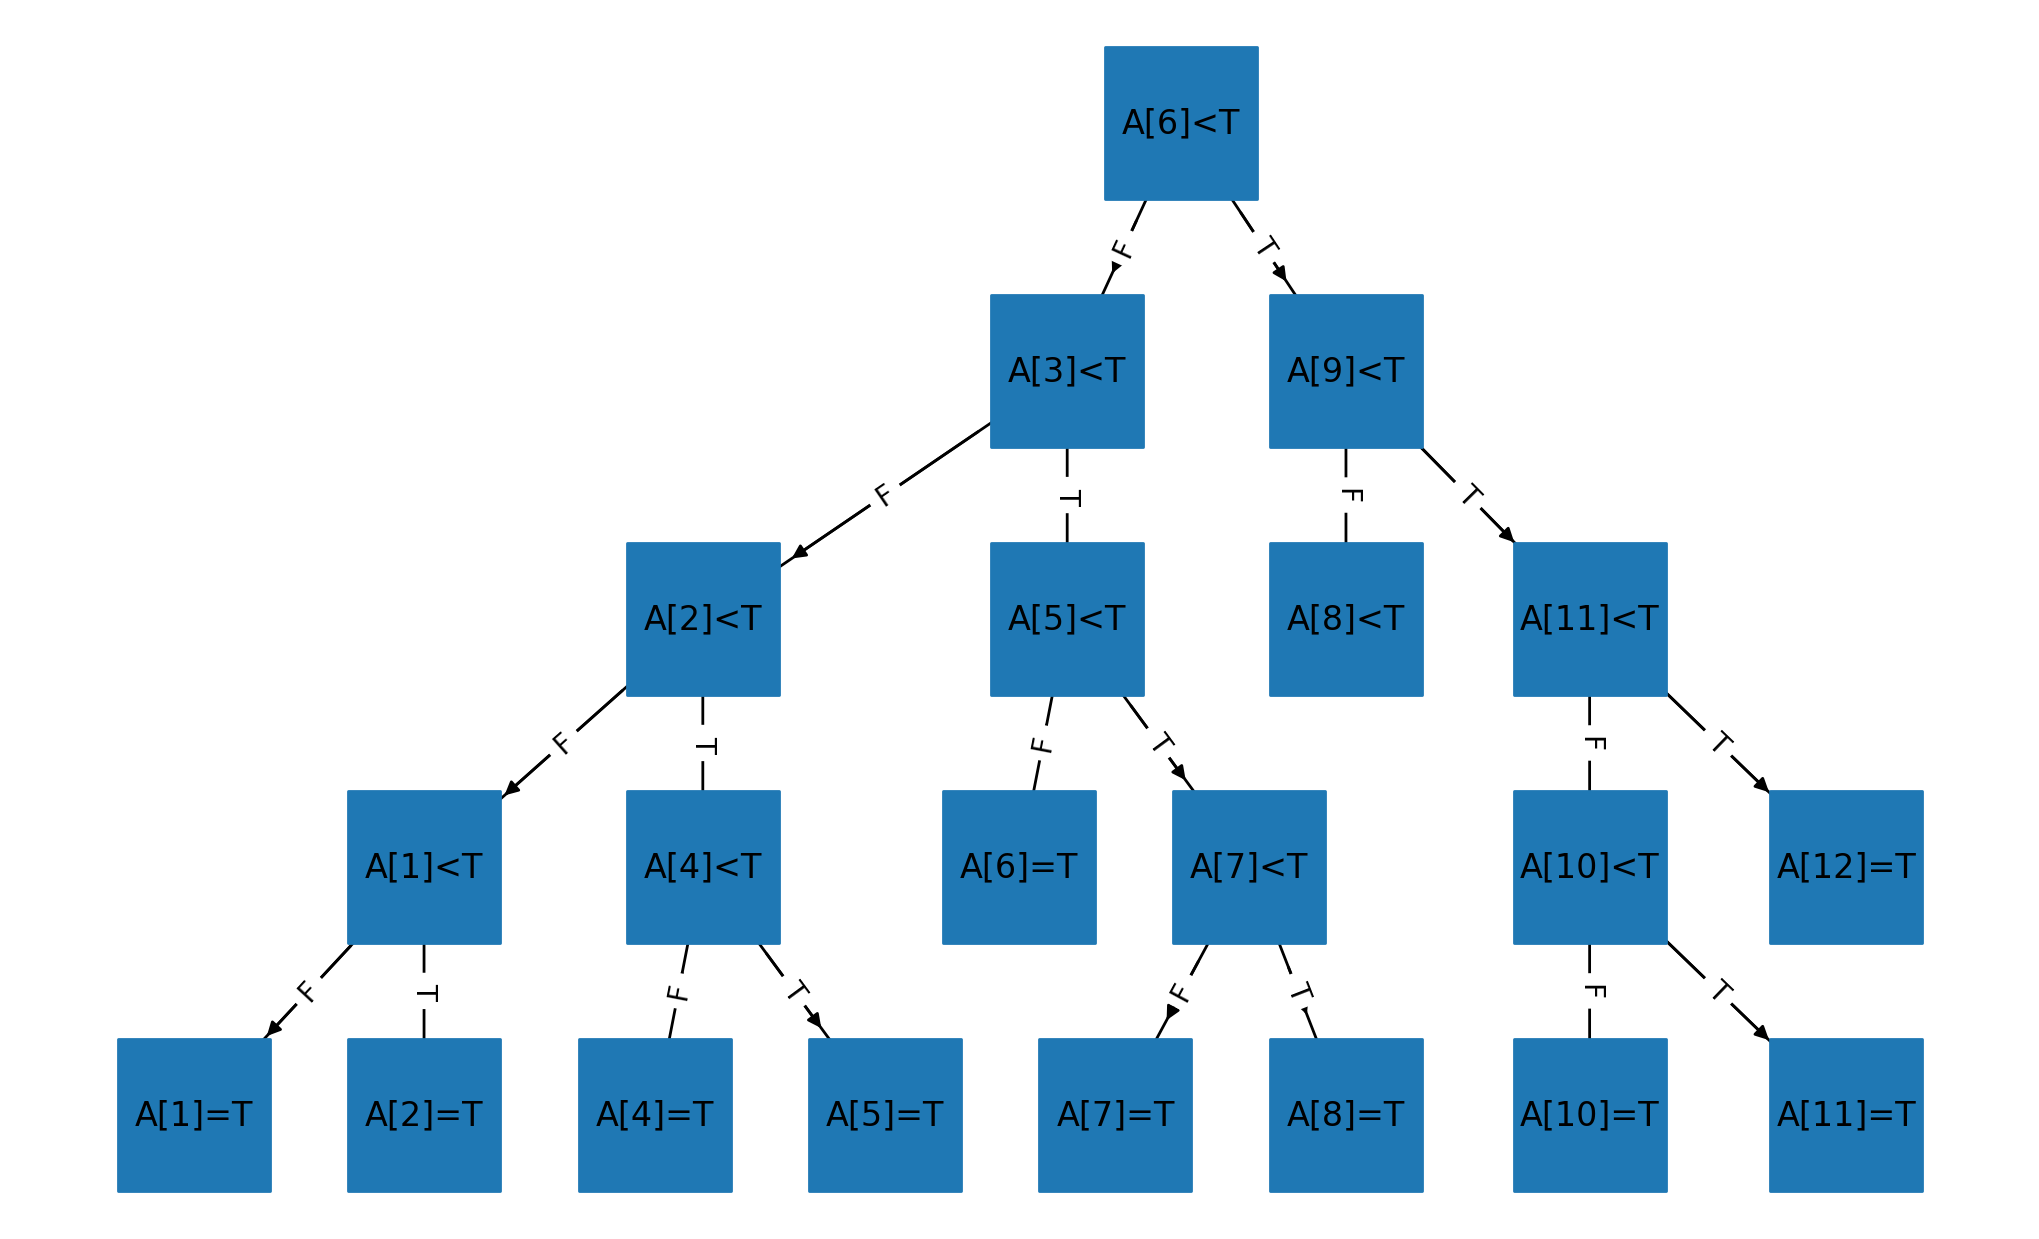
\includegraphics[width = 1\textwidth]{v2bintree.png}
        \caption{Binary Search V2 with $n=12$}
    \end{figure}
    This diagram is also a Binary Tree. But in it, from every internal vertex, there
    are exactly two edges downward in the diagram (never just one). This kind of
    Binary Tree is said to be a full Binary Tree. We will look into trees in detail in the next section.
    \begin{theorem}
        If \( T \) is a full binary tree with \( m \) internal vertices, then \( T \) has \( m + 1 \) leaves.
        \end{theorem}
        
        \begin{proof}
        We proceed by induction on the number of internal vertices, \( m \).
        
        \textbf{Base Case:} When \( m = 1 \), there is only one internal vertex, which is the root of the tree. By the definition of a full binary tree, the root must have two children, and since these children cannot be internal vertices (as there is only one internal vertex, the root itself), they must be leaves. Hence, the tree has \( 1 + 1 = 2 \) leaves, which satisfies our theorem.
        
        \textbf{Inductive Step:} Assume that the theorem holds for a full binary tree with \( m \) internal vertices, such that the tree has \( m + 1 \) leaves. Now consider a full binary tree with \( m + 1 \) internal vertices. By the definition of a full binary tree, adding an internal vertex means we are adding two children to an existing leaf (which is now converted into an internal vertex). This addition results in one less leaf (the converted internal vertex) and two more leaves (the new children). Therefore, the number of leaves increases by \( 2 - 1 = 1 \) compared to the number of leaves in the tree with \( m \) internal vertices.
        
        So, a tree with \( m + 1 \) internal vertices will have \( (m + 1) + 1 \) leaves. Hence, by the principle of mathematical induction, the theorem is true for all \( m \geq 1 \).
        \end{proof}
    \subsection{Exercises}
    \begin{exercise}
        Suppose \( T \) is not found by Binary Search. Where will \( T \) fit into the array? 
        Where should it be inserted?
    \begin{enumerate}
        \item Is the final \( q \)-value always one less than the final \( p \)-value?
        \item When is \( A[q] < T < A[p] \)?
        \item If \( p = 1 \) (that is, \( p \) was never changed), is \( T < A[1] \)?
        \item If \( q = n \) (that is, \( q \) was never changed), is \( A[n] < T \)?
    \end{enumerate}
    \end{exercise}
    
    \textbf{Solution}:
    \begin{enumerate}
        \item The final value of \( q \) is not necessarily always one less than the final \( p \) value. It depends on the search process and the position where \( T \) would fit if it were in the array.
        \item The condition \( A[q] < T < A[p] \) holds when \( T \) would be inserted between \( A[q] \) and \( A[p] \) in a sorted array to maintain the sorted order.
        \item If \( p = 1 \), it means \( T < A[1] \), and \( T \) should be inserted at the beginning of the array.
        \item If \( q = n \), it means \( A[n] < T \), and \( T \) should be inserted at the end of the array.
    \end{enumerate}


    \begin{exercise}
        Consider the best performance of binary search in $\Theta$ notation and worst performance in big $O$ notation. Is it possible to get the average performance in $\Theta$ notation? If yes, state the precise time complexity; if not, explain why.
    \end{exercise}
    \textbf{Solution:}

    \begin{itemize}
        \item Best time complexity: The best case scenario occurs when the target value is at the midpoint of the array, which happens with a constant time complexity, thus $\Omega(1)$. However, best case scenarios are generally not described using $\Theta$ notation as it implies a tight bound that is both the upper and lower limit, which is not applicable for the best case.
        \item Worst time complexity: Binary search has a worst-case time complexity of $O(\log n)$ when the target value is not within the initial bounds of the midpoint checks, thus requiring the maximum number of iterations to converge on the target.
        \item Average time complexity: The average time complexity of binary search is generally represented as $O(\log n)$. This is due to the fact that, on average, the number of steps required to find an element in a sorted array is logarithmic relative to the array size. Precise average case analysis of binary search is complex as it depends on the probability distribution of the target element's position. It is generally not represented in $\Theta$ notation because the lower and upper bounds for the average case cannot be tightly bounded as they can be for the best and worst cases.
    \end{itemize}
    
    \begin{exercise}
        Prove by MI that $\displaystyle \forall \ k\in \mathbb{N} ,\ $if Binary Search is applied to an array of length$\displaystyle \ n$ and has not terminated after $\displaystyle k$ (unsuccessful) probes, then the length of the current sublist must be less or equal to $\displaystyle \frac{n}{2^{k}}$
    \end{exercise}
    \begin{proof}
        We use $\displaystyle L(w)$ to denote the length of the current sublist after $\displaystyle w$ probes.
        
        \textbf{Base Case:}
        When $\displaystyle k=0$, the sorting is not yet started, so $\displaystyle L( 0) =n$, and we have $\displaystyle L( 0) =\frac{n}{2^{0}} =n$.
        
        \textbf{Inductive hypothesis:}
        Now assume that when $\displaystyle k=w$, it holds that:
        \begin{equation*}
        L( w) \leq \frac{n}{2^{w}}
        \end{equation*}
        
        \textbf{Inductive Step:}
        Thus, we need to prove that for $\displaystyle k=w+1$, $\displaystyle L( w+1) \leq 
        \frac{n}{2^{w+1}}$.
        We have proven earlier in theorem \ref{4.2.1} that after $\displaystyle w$ loops, $\displaystyle 
        \lfloor n/2^{w} \rfloor \leq L( w) \leq \lceil n/2^{w} \rceil $, and the length of the 
        sublist to be probed after $\displaystyle k+1$ unsuccessful probes is $\displaystyle 
        \frac{n}{2^{w+1}}$. While \ $\displaystyle \frac{n}{2^{w+1}} \leq \lceil n/2^{w+1} \rceil $. 
        Refer to the definition of $\displaystyle w( k)$ in the statement of problem, $\displaystyle 
        w\in \mathbb{N}$, so $\displaystyle \frac{n}{2^{w+1}} =\lceil n/2^{w+1} \rceil \ $. Hence, $\displaystyle L( w+1) \ \leq \frac{n}{2^{w+1}} \ $, this completes the proof.
    \end{proof}
    
\end{comment}

